\documentclass{report}

\input{~/dev/latex/template/preamble.tex}
\input{~/dev/latex/template/macros.tex}

\title{\Huge{}}
\author{\huge{Nathan Warner}}
\date{\huge{}}
\pagestyle{fancy}
\fancyhf{}
\lhead{Warner \thepage}
\rhead{}
% \lhead{\leftmark}
\cfoot{\thepage}
\setborder
% \usepackage[default]{sourcecodepro}
% \usepackage[T1]{fontenc}

\begin{document}
    % \maketitle
        \begin{titlepage}
       \begin{center}
           \vspace*{1cm}
    
           \textbf{Chapters 9-12} \\
    
           \vspace{0.5cm}
           Stat 128: Elementary Statistics
            
                
           \vspace{1.5cm}
    
           \textbf{Nathan Warner}
    
           \vfill
                
                
           \vspace{0.8cm}
         
           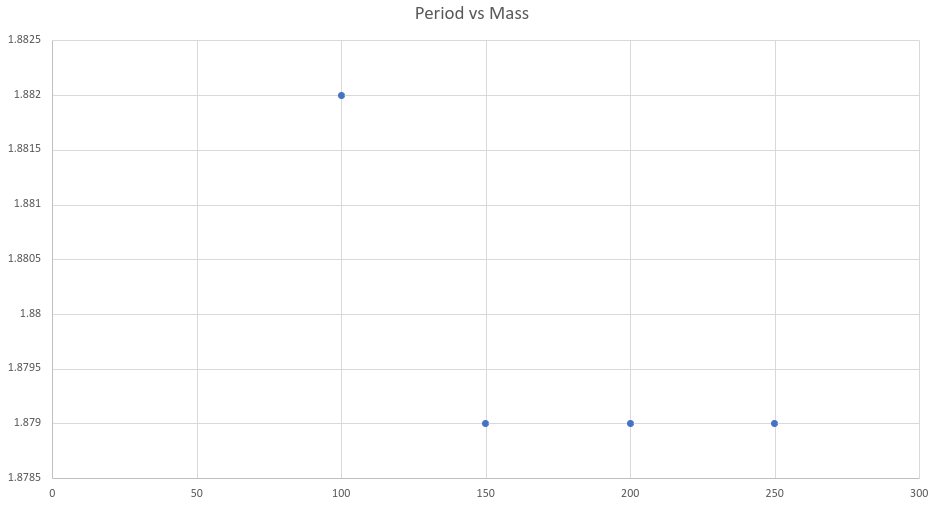
\includegraphics[width=0.4\textwidth]{/home/datura/dormprep/figures/1.png}
                
           Computer Science \\
           Northern Illinois University\\
           United States\\
           July 27, 2023
           
                
       \end{center}
    \end{titlepage}
    \tableofcontents
    \pagebreak \bigbreak \noindent
    \begin{center}
        \phantomsection
        \addcontentsline{toc}{section}{Chapter 9}
        \section*{Chapter 9}
    \end{center}
    \line(1,0){490}
    \bigbreak \noindent 
    \subsection{9.1 Estimating a Population Proportion}
    \bigbreak \noindent \bigbreak \noindent  
    \textbf{\textit{\underline{Learning Objectives For This Section:}}}
    \begin{enumerate}
        \item \textbf{Obtain a Point Estimate for the Population Proportion}
        \item \textbf{Construct and Interpret a Confidence Interval for the Population Proportion}
        \item \textbf{Determine the Sample Size Necessary for Estimating a Population Proportion within a Specified Margin of Error}
    \end{enumerate}
    \bigbreak \noindent \bigbreak \noindent 
    \textbf{Vocab:}
    \begin{itemize}
        \item A \textbf{point estimate} is the value of a statistic that estimates the value of a parameter.
        \item \textbf{A Confidence Interval} for an  unknown parameter consists of an interval of numbers based on a point estimate.
        \item \textbf{The level of confidence} represents the expected proportion of intervals that will contain the parameter if a large number of different samples is obtained.
        \item \textbf{Critical Value} represents the number of standard deviations the sample statistic can be from the parameter and still result in an interval that includes the parameter.
    \end{itemize}
    \bigbreak \noindent \bigbreak \noindent 
    \textbf{Formulas/Notation:}
    \begin{itemize}
        \item \textbf{Point Estimate = Sample Proportion}
            \begin{align*}
                \hat{p} = \frac{x}{n}
            .\end{align*}
        \item The \textbf{Margin of Error} is denoted:
            \begin{align*}
                E 
            .\end{align*}
        \item \textbf{Confidence Intervals for a Proportion} are of the form:
            \begin{center}
                point estimate $\pm $ margin of error
            \end{center}
            That is:
            \begin{align*}
               \hat{p} \pm E 
            .\end{align*}
            We have 95\% confidence that the sampling proportion will lie between:
            \begin{align*}
                \hat{p} \pm 1.96 \sigma_{\hat{p}}  
            .\end{align*}
        \item \textbf{The level of confidence} is denoted:
            \begin{align*}
                (1-\alpha) \cdot 100\%
            .\end{align*}
        \item \textbf{Standard Error:}
            \begin{align*}
                \sigma_{\hat{p}} = \sqrt{\frac{\hat{p}(1-\hat{p})}{n}}
            .\end{align*}
        \item \textbf{Constructing any (1−$\alpha $)$\cdot  $100\% Confidence Interval}
            \begin{align*}
                \hat{p} - z_{\alpha/2} \cdot \sqrt{\frac{\hat{p}(1-\hat{p})}{n}} < p < \hat{p} + z_{\alpha/2} \cdot \sqrt{\frac{\hat{p}(1-\hat{p})}{n}}
            .\end{align*}

        \item \textbf{Critical Value}
            \begin{align*}
                z_{ \frac{\alpha}{2}}
            .\end{align*}
            \bigbreak \noindent \bigbreak \noindent
        \end{itemize}

        \pagebreak \bigbreak \noindent 
        \begin{itemize}
            \item  \textbf{Constructing a (1−$\alpha $)$\cdot$ 100\% Confidence Interval for a Population Proportion:}
            Suppose that a simple random sample of size $n $ is taken from a population or the data are the result of a randomized experiment. A (1−$\alpha $)$\cdot  $100\% confidence interval for $p $ is given by the following quantities:
          \begin{align*}
              Lower\ bound:\ \hat{p} - z_{\frac{\alpha}{2}} \cdot \sqrt{\frac{\hat{p}(1 - \hat{p})}{n}}  \\
              Upper\ bound:\ \hat{p} + z_{\frac{\alpha}{2}} \cdot \sqrt{\frac{\hat{p}(1 - \hat{p})}{n}}
          .\end{align*}
          \textbf{Note:} It must be the case that $n\hat{p}(1-\hat{p})\geq 10$ and $n \leq 0.05N$ to construct this interval. Use $\hat{p}$ in place of $p$ in the standard deviation. This is because $p$ is unknown, and $\hat{p}$ is the best point estimate of $p$.
          \item The \textbf{margin of error}, $E $, in a (1−$\alpha $)$\cdot  $100\% confidence interval for a population proportion is given by
          \begin{align*}
              E = Z_{\frac{\alpha}{2}} \cdot \sqrt{\frac{\hat{p}(1-\hat{p})}{n}} \\
              or:\ \frac{Upper\ Limit\ - Lower\ Limit}{2}
          .\end{align*}
      \item \textbf{Sample Size Needed for Estimating the Population Proportion}
          \begin{align*}
              n = \hat{p} \cdot (1 - \hat{p}) \cdot \left(\frac{z_{\alpha/2}}{E}\right)^2 
          .\end{align*}
          (rounded up to the next integer) where $\hat{p}$ is a prior estimate of p.
          \bigbreak \noindent 
          If a prior estimate of p is unavailable, the sample size required is
          \begin{align*}
              n = 0.25 \cdot \left(\frac{z_{\alpha/2}}{E}\right)^2
          .\end{align*}
          rounded up to the next integer. The margin of error should always be expressed as a decimal when using these formulas.
        \item \textbf{Width}
            \begin{align*}
                2(E)
            .\end{align*}
      \end{itemize}


    \pagebreak \bigbreak \noindent 
    \textbf{\textit{\underline{Introduction}}}
    \bigbreak \noindent 
    \textbf{Two Types of Inferential Statistics:}
    \begin{enumerate}
        \item Estimation
        \item Hypothesis Testing
    \end{enumerate}

    \bigbreak \noindent \bigbreak \noindent 
    \textbf{\textit{\underline{Obtain a Point Estimate for the Population Proportion}}}
    \bigbreak \noindent 
    Suppose we want to estimate the proportion of adult Americans who believe that the amount they pay in federal income taxes is fair. It is unreasonable to expect that we could survey every adult American. Instead, we use a sample of adult Americans to arrive at an estimate of the proportion. We call this estimate a point estimate.
    \bigbreak \noindent 
    \begin{mdframed}
      \textbf{Example: }
      \bigbreak \noindent 
      \textbf{Problem:}
      \bigbreak \noindent 
      The Gallup Organization conducted a poll in April 2017 in which a simple random sample of 1019 Americans aged 18 and older were asked, “Do you regard the income tax that you will have to pay this year as fair?” Of the 1019 adult Americans surveyed, 620 said yes. Obtain a point estimate for the proportion of Americans aged 18 and older who believe that the amount of income tax they pay is fair.
      \bigbreak \noindent 
      \textbf{Approach:}
      The point estimate of the population proportion is $\hat{p}=\frac{x}{n}$, where $x=620$ and $n=1019$.
      \bigbreak \noindent 
      \textbf{Solution:}
      \bigbreak \noindent 
      Substituting into the formula, we get $\hat{p}=\frac{x}{n}=\frac{620}{1019}=0.608=60.8\%$.
      \bigbreak \noindent 
        We estimate that 60.8\% of Americans aged 18 and older believe that the amount of income tax they pay is fair.
    \end{mdframed}

    \bigbreak \noindent \bigbreak \noindent 
    \textbf{\textit{\underline{Construct and Interpret a Confidence Interval for the Population Proportion}}}
    \bigbreak \noindent 
    What if we conducted a different random sample of 1019 Americans aged 18 years or older? Would we get the same sample proportion who believe the amount of income tax they pay is fair? Probably not. Why? Because statistics such as $\hat{p}$ vary from sample to sample. So a different random sample of adult Americans might result in a different point estimate of the population proportion, such as $\hat{p}=0.593$.
    \bigbreak \noindent 
    If the method used to select the adult Americans was done appropriately, both point estimates would be good guesses of the population proportion. Due to variability in the sample proportion, we report a range (or interval) of values, including a measure of the likelihood that the interval includes the unknown population proportion.
    \bigbreak \noindent
    Consider the following:
    \begin{align*}
        \hat{p} = 0.54 \quad E = 0.034
    .\end{align*}
    Then:
    \begin{align*}
        0.54 - 0.034 = 0.506 \\
        0.54 + 0.034 = 0.574
    .\end{align*}
    With this we can say "We are 95\% confident that the proportion is between 0.506 and 0.574"
    \pagebreak \bigbreak \noindent 
    Figure:
    \bigbreak \noindent \bigbreak \noindent 
    \begin{figure}[ht]
        \centering
        \incfig{figmanea}
        \label{fig:figmanea}
    \end{figure}
    \bigbreak \noindent 
    Where does the 1.96 comes from?
    \begin{align*}
        z_{\alpha} \\
        z_{0.025} = 1.96
    .\end{align*}
    \bigbreak \noindent \bigbreak \noindent 
    This graphic also infers that 95\% of all sample proportions will lie between:
    \begin{align*}
        p-1.96\sigma_{\hat{p}} < \hat{p} < p +1.96\sigma_{\hat{p}}
    .\end{align*}
    \bigbreak \noindent \bigbreak \noindent 
    By solving this inequality such that $p $ is in the center:
    \begin{align*}
        \hat{p} -1.96\sigma_{\hat{p}} < p < \hat{p}  + 1.96 \sigma_{\hat{p}}
    .\end{align*}
    \bigbreak \noindent 
    And we can write this in shorthand form:
    \begin{align*}
        \hat{p} \pm 1.96 \sigma_{\hat{p}} \\
        or:\ \hat{p} \pm E
    .\end{align*}
    \bigbreak \noindent 
    \textit{figure:}
    \bigbreak \noindent 
\begin{figure}[ht]
    \centering
    \incfig{fuga}
    \label{fig:fuga}
\end{figure}

    \pagebreak \bigbreak \noindent 
    \textbf{Summary:}
    \bigbreak \noindent 
    \begin{itemize}
        \item for a 95\% confidence interval, any sample proportion that lies withing 1.96 standard errors of the population proportion will result in a confidence interval that includes $p $. This will happen in 95\% of all possible samples.
        \item Any sample proportion that is more than 1.96 standard errors from the population proportion will result in a confidence interval that does not contain $p $. This will happen in 5\% of all possible samples (those sample proportions in the tails of the distribution).
        \item A confidence interval for an unknown parameter consists of an interval of numbers based on a point estimate.
        \item The level of confidence represents the expected proportion of intervals that will contain the parameter if a large number of different samples is obtained. The level of confidence is denoted (1−$\alpha $)$\cdot $ 100\%.
        \item Whether a confidence interval contains the population parameter depends solely on the value of the sample statistic. Any sample statistic that is in the tails of the sampling distribution will result in a confidence interval that does not include the population parameter. See Figure 1. Notice that $\hat{p}_1$ results in a confidence interval that includes the population proportion, $p$. However, $\hat{p}_2$ results in a confidence interval that does not include the population proportion, $p$, because $\hat{p}_2$ is in the tails of the distribution.
    \end{itemize}

    \bigbreak \noindent \bigbreak \noindent 
    \qs{}{The horizontal axis in the sampling distribution of  represents all possible sample proportions from a simple random sample of size n. 
        \bigbreak \noindent 
        \textbf{a.) What percent of sample proportions results in a ​75\% confidence interval that includes the population​ proportion?}
        \smallbreak \noindent
        \textbf{b.) What percent of sample proportions results in a ​75\% confidence interval that does not include the population​ proportion?}
        \bigbreak \noindent 
        \pf{Solution:}{}
        \textbf{a.)} 75\%
        \smallbreak \noindent
        \textbf{b.)} 25\%
}
    \bigbreak \noindent 
    \textbf{Caution:}
    \bigbreak \noindent 
    95\% confident does not mean 95\% probability. Probability describes the likelihood of undetermined event.
    \bigbreak \noindent 
    It does not make sense to talk about the probability that the interval contains the parameter, because the parameter is an unknown, but fixed value. Thus, it is either in the interval, or not. 
    \bigbreak \noindent 
    Consider a coin flip, if a coin has been flipped but its outcome has not been revealed, the flip resulting in a head is not $\frac{1}{2} $, because the outcome has already been determined. Instead the probability is either $0$, or $1$
    \bigbreak \noindent 
    Therefore, the probability that any confidence interval contains a parameter is either $0$, or $1$.
    \bigbreak \noindent 
    We do say "we are 95\% confident the interval contains the parameter" because the method "works" in 95\% of all samples.

    \pagebreak \bigbreak \noindent 
    \textbf{Constructing any $(1-\alpha)\cdot 100\% $ Confidence interval}
    \bigbreak \noindent 
    We need a method for constructing any $(1-\alpha) \cdot 100\%$ confidence interval. When $\alpha=0.05$, we are constructing a $95\%$ confidence interval.
    \bigbreak \noindent 
    We generalize
    \begin{figure}[ht]
        \centering
        \incfig{construct}
        \label{fig:construct}
    \end{figure}
    \bigbreak \noindent 
    by first noting that $(1-\alpha)\cdot 100\%$  of all sample proportions are in the interval as shown in Figure 2.
    \bigbreak \noindent 
    \textit{Figure 2}
    \bigbreak \noindent 
    \begin{figure}[ht]
        \centering
        \incfig{const}
        \label{fig:const}
    \end{figure}
    \bigbreak \noindent 
    Rewrite this inequality with p in the middle and obtain
    \begin{align*}
        \hat{p} - z_{\frac{\alpha}{2}} \cdot \sqrt{\frac{\hat{p}(1 - \hat{p})}{n}} < p < \hat{p} + z_{\frac{\alpha}{2}} \cdot \sqrt{\frac{\hat{p}(1 - \hat{p})}{{n}}}
    .\end{align*}
    \bigbreak \noindent 
    So (1−$\alpha $)⋅100\% of all sample proportions will result in confidence intervals that contain the population proportion. The sample proportions that are in the tails of the distribution in Figure 2 will not result in confidence intervals that contain the population proportion.

    \pagebreak \bigbreak \noindent 
    Table 1 shows some of the common critical values used in the construction of confidence intervals. Notice that higher levels of confidence correspond to higher critical values. After all, if your level of confidence that the interval includes the unknown parameter increases, the width of your interval (through the margin of error) should increase.
    \begin{center}
        \begin{center}
            \begin{tabular}{|l|c|c|}
            \hline
            Level of confidence $(1-\alpha) \cdot 100\%$ & Area in each tail $\frac{\alpha}{2}$ & Critical Value $z_{\frac{\alpha}{2}}$ \\
            	\hline
            90\% & 0.05 & 1.645   \\
            	\hline
            95\% & 0.025 & 1.96 \\
            \hline 
            99\% & 0.005 & 2.575 \\
            \hline
            \end{tabular}
        \end{center}
    \end{center}

    \bigbreak \noindent 
    \textbf{Interpretation of a Confidence Interval }
    \bigbreak \noindent 
    A $(1-\alpha)\cdot 100\%$ confidence interval indicates that $(1-\alpha)\cdot 100\%$ of all simple random samples of size $n$ from the population whose parameter is unknown will result in an interval that contains the parameter.
    \bigbreak \noindent 
    For example, a 90\% confidence interval for a parameter suggests that 90\% of all possible samples will result in an interval that includes the unknown parameter and 10\% of the samples will result in an interval that does not capture the parameter.
    \begin{mdframed}
      \textbf{Example: Interpreting a Confidence Interval}
      \bigbreak \noindent 
      \textbf{Problem:}
      The Gallup Organization conducted a poll in April 2017 in which a simple random sample of 1019 Americans aged 18 and older were asked, “Do you regard the income tax that you will have to pay this year as fair?” We learned from Example 1 that the proportion of those surveyed who responded yes was 0.608. Gallup reported its “survey methodology” as follows:
      \bigbreak \noindent 
      \textbf{Approach:}
      Confidence intervals for a proportion are of the form point estimate ± margin of error. So add and subtract the margin of error from the point estimate to obtain the confidence interval. Interpret the confidence interval, ”We are 95\% confident that the proportion of Americans aged 18 and older who believe that the income tax they will have to pay this year is fair is between lower bound and upper bound.”
      \bigbreak \noindent 
      \textbf{Solution:}
      \bigbreak \noindent 
      The point estimate is 0.608, and the margin of error is 0.04. The confidence interval is $0.608 \pm 0.04$. Therefore, the lower bound of the confidence interval is $0.608 - 0.04 = 0.568$ and the upper bound of the confidence interval is $0.608 + 0.04 = 0.648$. We are 95\% confident that the proportion of Americans aged 18 and older who believe that the income tax they will have to pay this year is between 0.568 and 0.648.
      \bigbreak \noindent 
    \end{mdframed}
    \bigbreak \noindent 
      \textbf{We are now prepared to present a method for constructing a confidence interval about the population proportion, $p $}
      \bigbreak \noindent 
      \textbf{Constructing a (1−$\alpha $)⋅100\% Confidence Interval for a Population Proportion:}
      \bigbreak \noindent 
      Suppose that a simple random sample of size $n $ is taken from a population or the data are the result of a randomized experiment. A (1−$\alpha $)⋅100\% confidence interval for $p $ is given by the following quantities:
      \begin{align*}
          Lower\ bound:\ \hat{p} - z_{\frac{\alpha}{2}} \cdot \sqrt{\frac{\hat{p}(1 - \hat{p})}{n}}  \\
          Upper\ bound:\ \hat{p} + z_{\frac{\alpha}{2}} \cdot \sqrt{\frac{\hat{p}(1 - \hat{p})}{n}}
      .\end{align*}
      \bigbreak \noindent 
      \nt{It must be the case that $n\hat{p}(1-\hat{p})\geq 10$ and $n \leq 0.05N$ to construct this interval. Use $\hat{p}$ in place of $p$ in the standard deviation. This is because $p$ is unknown, and $\hat{p}$ is the best point estimate of $p$.}

      \pagebreak \bigbreak \noindent 
      \bigbreak \noindent 
      \begin{mdframed}
        \textbf{Example: Constructing a Confidence Interval for a Population Proportion (Statcrunch)}
        \bigbreak \noindent 
        \textbf{Problem:}
        In the Parent–Teen Cell Phone Survey conducted by Princeton Survey Research Associates International, 800 randomly sampled 16- to 17-year-olds living in the United States were asked whether they have ever used their cell phone to text while driving. Of the 800 teenagers surveyed, 272 indicated that they text while driving. Obtain a 95\% confidence interval for the proportion of 16- to 17-year-olds who text while driving.
        \bigbreak \noindent 
        \textbf{Approach:}
        It is important to verify the requirements for constructing the confidence interval first. It must be the case that $n\hat{p}(1 −\hat{p}) \geq 10$ and the sample size is no more than 5\% of the population size (n $ \leq $0.05N).Then, construct the confidence interval either by hand or using technology.
        \bigbreak \noindent 
        \textbf{Solution:}
        \bigbreak \noindent 
        First, we obtain $\hat{p} $
        \begin{align*}
            \hat{p} = \frac{272}{800} = .34
        .\end{align*}
        \bigbreak \noindent 
        Verify Necessary Conditions:
        \begin{align*}
           n\hat{p}(1-\hat{p})  \geq 10 \\
            800(.34)(.66) = 179.52 \geq 10
        .\end{align*}
        \bigbreak \noindent 
        Also, we know that $n \leq0.05N $:
        \bigbreak \noindent 
        now in statcrunch:
        \begin{enumerate}
            \item Stat $>$ Proportion Stats $> $ One Sample $> $ with summary
            \item Input no. of successes
            \item Input no. of observations
            \item Input confidence level
            \item Method: Standard-Wald
            \item Compute
        \end{enumerate}
        \bigbreak \noindent 
        after doing the StatCrunch steps, we get a result of 0.307 and 0.373, therefore, we can conclude that we are 95\% confident that the proportion of 16 to 17-year-olds who text while driving is between 0.307 and 0.373

      \end{mdframed}

      \pagebreak \bigbreak \noindent 
        \begin{mdframed}
        \textbf{Example: Constructing a Confidence Interval for a Population Proportion (By hand)}
        \bigbreak \noindent 
        \textbf{Problem:}
        In the Parent–Teen Cell Phone Survey conducted by Princeton Survey Research Associates International, 800 randomly sampled 16- to 17-year-olds living in the United States were asked whether they have ever used their cell phone to text while driving. Of the 800 teenagers surveyed, 272 indicated that they text while driving. Obtain a 95\% confidence interval for the proportion of 16- to 17-year-olds who text while driving.
        \bigbreak \noindent 
        \textbf{Approach:}
        It is important to verify the requirements for constructing the confidence interval first. It must be the case that $n\hat{p}(1 −\hat{p}) \geq 10$ and the sample size is no more than 5\% of the population size (n $ \leq $0.05N).Then, construct the confidence interval either by hand or using technology.
        \bigbreak \noindent 
        \textbf{Solution:}
        \bigbreak \noindent 
        First, we obtain $\hat{p} $
        \begin{align*}
            \hat{p} = \frac{272}{800} = .34
        .\end{align*}
        \bigbreak \noindent 
        Verify Necessary Conditions:
        \begin{align*}
           n\hat{p}(1-\hat{p})  \geq 10 \\
            800(.34)(.66) = 179.52 \geq 10
        .\end{align*}
        \bigbreak \noindent 
        Also, we know that $n \leq0.05N $:
        \bigbreak \noindent 
        Now, to use the formula:
        \begin{align*}
            \hat{p} \pm E \\
        Where\ E = z_{\frac{\alpha}{2}} \cdot \sqrt{\frac{\hat{p}(1-\hat{p})}{n}}
        .\end{align*}
        We will need to find alpha, given that the formula for confidence level is:
        \begin{align*}
            (a-\alpha) \cdot 100\% \\
            1- \alpha = 0.95 \\
            \alpha = 0.05
        .\end{align*}
        \bigbreak \noindent 
        So our critical value is:
        \begin{align*}
            z_{\frac{\alpha}{2}} = z_{\frac{0.05}{2}} \\
            = z_{0.025}
        .\end{align*}
        Using the normal distribution table, we get:
        \begin{align*}
            \alpha = 1.96
        .\end{align*}
        \bigbreak \noindent 
        Now we can compute our bounds:
        \begin{align*}
            LB:\ = \hat{p} - z_{\frac{\alpha}{2}} \cdot \sqrt{\frac{\hat{p}(1-\hat{p})}{n}} \\
            = 0.34 - 19.6 \cdot \sqrt{\frac{0.34(0.66)}{800}} \\
            = 0.307 \\
            UB = \hat{p} + z_{\frac{\alpha}{2}} \cdot \sqrt{\frac{\hat{p}(1-\hat{p})}{n}} \\
            =0.34 + 1.96 \cdot \sqrt{\frac{0.34(0.66)}{800}} \\
            = 0.373
        .\end{align*}
        \bigbreak \noindent 
        Therefore:
        \begin{align*}
            Upper\ bound:\ 0.307 \quad Upper\ Bound:\ 0.373 \\
            Or: (0.307,0.373)
        .\end{align*}

    \end{mdframed}


    \bigbreak \noindent \bigbreak \noindent 
      \textbf{The Effect of Level of Confidence on the Margin of Error}
      \bigbreak \noindent 
      \begin{mdframed}
          \textbf{Example: The Role of the Level of Confidence in the Margin of Error} 
          \bigbreak \noindent 
          \textbf{Problem:}
          In the Parent--Teen Cell Phone Survey conducted by Princeton Survey Research Associates International, 800 randomly sampled 16- to 17-year-olds living in the United States were asked whether they have ever used their cell phone to text while driving. Of the 800 teenagers surveyed, 272 indicated that they text while driving. From the last example, we concluded that we are 95\% confident that the proportion of 16- to 17-year-olds who text while driving is between 0.307 and 0.373. Determine the effect on the margin of error by increasing the level of confidence from 95\% to 99\%.
          \bigbreak \noindent 
          \textbf{Approach:}
          We would expect the margin of error to increase with a larger level of confidence. Construct the confidence interval either by hand or using technology.
          \bigbreak \noindent 
          \textbf{Solution:}
          \bigbreak \noindent 
          The margin of error for the 95\% confidence interval found in Example 3 is 0.033, and the margin of error for the 99\% confidence interval is 0.043. So increasing the level of confidence increases the margin of error, resulting in a wider confidence interval.
      \end{mdframed}
      \bigbreak \noindent \bigbreak \noindent 
      \textbf{The Effect of Sample Size on the Margin of Error}
      \bigbreak \noindent 
      We know that larger sample sizes produce more precise estimates (the Law of Large Numbers). Given that the margin of error is $E=z_{\alpha/2} \cdot \hat{p} \cdot \sqrt{\frac{(1-\hat{p})}{n}}$, we can see that increasing the sample size $n$ decreases the standard error, so the margin of error decreases. Therefore, larger sample sizes will result in narrower confidence intervals.
      \bigbreak \noindent 
      \textbf{What If We Do Not Satisfy the Normality Condition?}
      \bigbreak \noindent 
     When the normality condition is not satisfied, the proportion of intervals that capture the parameter is below the level of confidence.

     \pagebreak \bigbreak \noindent 
     \textbf{\textit{Determine the Sample Size Necessary for Estimating a Population Proportion within a Specified Margin of Error}}
     \bigbreak \noindent 
     \begin{mdframed}
       \textbf{Example: Determining Sample Size}
       \bigbreak \noindent 
       \textbf{Problem:}
       An economist wants to know if the proportion of the U.S. population who commutes to work via car-pooling is on the rise. What size sample should be obtained if the economist wants an estimate within 2 percentage points of the true proportion with 90\% confidence?
       \bigbreak \noindent 
       Assume that the economist uses the estimate of 10\% obtained from the American Community Survey.
       \bigbreak \noindent 
       \textbf{Approach:}
       Since \(1 - \alpha = 0.9\), we know that \(\alpha = 0.10\). Use \(E = 0.02\), \(z_{\alpha/2} = z_{0.12} = z_{0.05} = 1.645\), and \(\hat{p} = 0.10\) (the prior estimate).
       \bigbreak \noindent 
       \textbf{Solution:}
       Using the formula assuming that a prior estimate is available, \(n = \hat{p}(1 - \hat{p})\left(\frac{z_{\alpha/2}}{E}\right)^2\), we obtain
       \begin{align*}
           n = \hat{p}(1 - \hat{p})\left(\frac{z_{\alpha/2}}{E}\right)^2 = 0.10 \times (1 - 0.10) \times \left(\frac{1.645}{0.02}\right)^2 = 608.9 
       .\end{align*}
       Round this value up to 609. So the economist must survey 609 randomly selected residents of the United States.
       \bigbreak \noindent 
       \textbf{statcrunch steps:}
       \bigbreak \noindent 
       First:
       \begin{align*}
           E = 0.02\ (\text{The 2 percentage points}) \\
           W = 2(E) = 0.04 \\
           C.Level = 0.9 \\
           Target\ Proportion = 0.1
       .\end{align*}
       \begin{enumerate}
           \item Stats $>$ Proportion Stats $>$ One Sample $> $ Width/Sample Size
            \item Input confidence level
            \item Input Target Proportion
            \item Compute
       \end{enumerate}
       \bigbreak \noindent 
       And we find that the minimum sample size would be 609
       \bigbreak \noindent 
       Now consider that the economist does not use any prior estimates (target proportion), in this case, our target proportion will be 0.5
       \bigbreak \noindent 
       With this target proportion we get 1691
     \end{mdframed}

     \pagebreak \bigbreak \noindent 
     \subsection{9.2: Estimating a Population Mean}
     \bigbreak \noindent 
     \textbf{\textit{\underline{Learning Objectives For This Section:}}}
     \begin{enumerate}
         \item \textbf{Obtain a Point Estimate for the Population Mean}
         \item \textbf{State Properties of Student’s t-Distribution}
         \item \textbf{Determine t-Values}
         \item \textbf{Construct and Interpret a Confidence Interval for a Population Mean}
         \item \textbf{Determine the Sample Size Necessary for Estimating a Population Mean within a Given Margin of Error}
     \end{enumerate}
     \bigbreak \noindent 
     \textbf{Vocab:}
     \begin{itemize}
         \item \textbf{The point estimate of the population mean}, $\mu$, is the sample mean, $\overline{x}$.
         \item \textbf{T-Interval:} confidence interval that uses the t-distribution
     \end{itemize}
     \bigbreak \noindent 
     \textbf{Notation/Formulas:}
     \begin{itemize}
        %  \item \textbf{Margin of error for population mean} 
        %      \begin{align*}
        %          z_{\frac{\alpha}{2}} \cdot \frac{\sigma}{\sqrt{n}}
        %      .\end{align*}
        % \item \textbf{Confidence Interval for population mean}
        %     \begin{align*}
        %         Point\ Estimate - Margin\ of\ Error \\
        %         = \overline{x} \pm z_{\frac{\alpha}{2}} \cdot \frac{\sigma}{\sqrt{n}} \\
        %         Or\ most\ likely = \overline{x} \pm z_{\frac{\alpha}{2}} \cdot \frac{s}{\sqrt{n}} \\
        %     .\end{align*}
        \item \textbf{Student’s t-distribution}
            \begin{align*}
               t = \frac{\overline{x}-\mu}{\frac{s}{\sqrt{n}}} 
            .\end{align*}
        \item \textbf{Constructing a (1−$\alpha $) $ \cdot $100\% Confidence Interval for $\mu$}
            Provided:
            \begin{itemize}
                \item sample data come from a simple random sample or randomized experiment
                \item sample size is small relative to the population size (n $ \leq $0.05N)
                \item the data come from a population that is normally distributed with no outliers, or the sample size is large
            \end{itemize}
            A (1−$\alpha $)$\cdot$100\% confidence interval for $\mu$ is given by
            \begin{align*}
                LB:\ = \overline{x}  - t_{\frac{\alpha}{2}} \cdot \frac{s}{\sqrt{n}} \\
                UB:\ = \overline{x}  + t_{\frac{\alpha}{2}} \cdot \frac{s}{\sqrt{n}} \\
            .\end{align*}
            where $t_{\frac{\alpha}{2}} $ is the critical value with n−1 degrees of freedom.
        \item \textbf{Margin of Error:}
            \begin{align*}
                E = t_{\frac{\alpha}{2}} \cdot \frac{s}{\sqrt{n}}
            .\end{align*}
        \item \textbf{Determine the Sample Size Necessary for Estimating a Population Mean within a Given Margin of Error}
            \begin{align*}
                n = \bigg(\frac{\frac{z_{\alpha}}{2}\cdot s}{E}\bigg)^{2}
            .\end{align*}
     \end{itemize}
     \pagebreak \bigbreak \noindent 
     \textbf{\textit{\underline{Obtain a Point Estimate for the Population Mean}}}
     \bigbreak \noindent 
     To find the point estimate of the population mean, compute the sample mean, $\overline{x} $

     \bigbreak \noindent \bigbreak \noindent 
     \textbf{\textit{\underline{State Properties of Student’s t-Distribution}}}
     \bigbreak \noindent 
     a different random sample of 16 cars would likely result in a different point estimate of $\mu$. For this reason, we want to construct a confidence interval for the population mean, just as we did for the population proportion.
     \bigbreak \noindent 
     A confidence interval for the population mean is of the form
     \begin{center}
         Point estimate $\pm $ Margin of Error
     \end{center}
     \bigbreak \noindent 
     (just like the confidence interval for a population proportion). To determine the margin of error, we need to know the sampling distribution of the sample mean.
     \bigbreak \noindent 
     Recall that the distribution of \(\bar{x}\) is approximately normal if the population from which the sample is drawn is normal or the sample size is sufficiently large. In addition, the distribution of \(\bar{x}\) has the same mean as the parent population, \(\mu_{\bar{x}} = \mu\), and a standard deviation equal to the parent population's standard deviation divided by the square root of the sample size, \(\sigma_{\bar{x}} = \frac{\sigma}{\sqrt{n}}\).
     \bigbreak \noindent 
     Following the same logic used in constructing a confidence interval about a population proportion, our confidence interval would be
     \begin{align*}
         point\ estimate \pm Margin\ of\ Error \\
         =  \bar{x} \pm z_{\frac{\alpha}{2}} \cdot \frac{\sigma}{\sqrt{n}}
     .\end{align*}
     \bigbreak \noindent 
     This presents a problem because we need to know the population standard deviation to construct this interval. It does not seem likely that we would know the population standard deviation but not know the population mean. So what can we do? A logical option is to use the sample standard deviation, \( s \), as an estimate of \( \sigma \). Then the standard deviation of the sampling distribution of \( \bar{x} \) would be estimated by \( \frac{s}{\sqrt{n}} \) and our confidence interval would be
     \begin{align*}
         \overline{x} \pm z_{\frac{\alpha}{2}} \cdot \frac{s}{\sqrt{n}}
     .\end{align*}
     \bigbreak \noindent 
     Unfortunately, there is a problem with this approach. The sample standard deviation, \( s \), is a statistic and therefore will vary from sample to sample. Using the normal model to determine the critical value, \( z_{\frac{\alpha}{2}} \), in the margin of error does not take into account the additional variability introduced by using \( s \) in place of \( \sigma \). This is not much of a problem for large samples because the variability in the sample standard deviation decreases as the sample size increases (Law of Large Numbers), but for small samples, we have a real problem.
     \bigbreak \noindent 
    Put another way, the z-score of \( \bar{x} \), \( \frac{\bar{x} - \mu}{\frac{\sigma}{\sqrt{n}}} \), is normally distributed with mean 0 and standard deviation 1 (provided \( \bar{x} \) is normally distributed). However, \( \frac{\bar{x} - \mu}{\frac{s}{\sqrt{n}}} \) is not normally distributed with mean 0 and standard deviation 1. So a new model must be used to determine the margin of error in a confidence interval that accounts for this additional variability. This leads to the story of William Gosset.
    \bigbreak \noindent 
    In the early 1900s, William Gosset worked for the Guinness brewery. Gosset was in charge of conducting experiments at the brewery to identify the best barley variety. When working with beer, Gosset was limited to small data sets. At the time, the model used for constructing confidence intervals about a mean was the normal model, regardless of whether the population standard deviation was known. Gosset did not know the population standard deviation, so he substituted the sample standard deviation for the population standard deviation and used the formula \(\bar{x} \pm z_{\frac{\alpha}{2}} \cdot \frac{s}{\sqrt{n}}\). While doing this, he was finding that his confidence intervals did not include the population mean at the rate expected. This led Gosset to develop a model that accounts for the additional variability introduced by using \( s \) in place of \( \sigma \) when determining the margin of error. Guinness would not allow Gosset to publish his results under his real name (Guinness was very secretive about its brewing practices), but did allow the results to be published under a pseudonym. Gosset chose "Student."

    \bigbreak \noindent 
    \begin{mdframed}
      \textbf{Definition: Student's T-Distribution}
      \bigbreak \noindent 
      We know that we can create a standard normal random variable, with the formula:
      \begin{align*}
          z = \frac{x - \mu}{s}
      .\end{align*}
      \bigbreak \noindent 
      Where $x $ is the value of the statistic, $\mu $ is the population mean, and $\sigma$ is the population standard deviation, Thus, if we wanted to created a standard normal random variable with a sample mean statistic, we would have the equation:
      \begin{align*}
          z = \frac{\overline{x} - \mu}{\frac{\sigma}{\sqrt{n}}}
      .\end{align*}
      \bigbreak \noindent 
      However this poses a problem, as states previously, we may not always know the value of $\sigma$, in this case, we can use students $t-distribution$, which states:
      \begin{align*}
           t = \frac{\overline{x} - \mu}{\frac{s}{\sqrt{n}}}
      .\end{align*}
      \bigbreak \noindent 
      So with the $t-distribution $, we are assuming we do not have access to $\sigma $.
      \bigbreak \noindent 
      It is important to note that when using students method, there will be additional variability in the $t-distribution$ compared to the $z-distribution $ 
    \end{mdframed}
    \bigbreak \noindent 
    \nt{Student's t-distribution is asymptotically normal, this means as the sample size n increases, student's t-distribution looks more and more like the standard normal distribution}

    \bigbreak \noindent 
    \textbf{Properties of the $t-distribution$}
    \begin{enumerate}
        \item The t-distribution is different for different degrees of freedom
        \item the t-distribution is centered at 0 and is symmetric about 0 
        \item The area under the curve is 1. The area around each curve to the right of 0 equals the area under the curve to the left of 0, which equals $1/2 $
     \item As t increases or decreases without bound, the graph approaches, but never equals, zero.
         \begin{align*}
             \lim\limits_{t \to -\infty}{f(x) = 0} \\
             \lim\limits_{t \to \infty}{f(x) = 0}
         .\end{align*}
        \item The area in the tails of the t-distribution is a little greater than the area in the tails of the standard normal distribution, because we are using $s $ as an estimate of $\sigma $, thereby introducing further variability into the t-statistic
        \item As the sample size $n $ increases, the density curve of $t $ get closer to the standard normal density curve. This result occurs because, as the sample size increases, the values of $s$ get closer to the value of $\sigma $, by the Law of Large Numbers.
    \end{enumerate}

    \pagebreak \bigbreak \noindent 
    \textbf{\textit{\underline{Construct and Interpret a Confidence Interval for a Population Mean}}}
    \bigbreak \noindent 
    We are now ready to construct a confidence interval for a population mean.
    \bigbreak \noindent 
    \textbf{Constructing a (1−$\alpha $)$\cdot $100\% Confidence Interval for $\mu$}
    \bigbreak \noindent 
    \textbf{Provided}
    \begin{itemize}
        \item sample data come from a simple random sample or randomized experiment
        \item sample size is small relative to the population size (n$\leq$0.05$N$)
        \item the data come from a population that is normally distributed with no outliers, or the sample size is large
    \end{itemize}
    \bigbreak \noindent 
    A (1−$\alpha$)$ \cdot  $100\% confidence interval for $\mu $ is given by:
    \begin{align*}
        Lower\ Bound:\ \overline{x} - t_{\frac{\alpha}{2}}\cdot \frac{s}{\sqrt{n}} \\
        Upper\ Bonud:\ \overline{x} + t_{\frac{\alpha}{2}}\cdot \frac{s}{\sqrt{n}} \\
    .\end{align*}
    \bigbreak \noindent 
    where $t_{\frac{\alpha}{2}} $ is the critical value with n−1 degrees of freedom.
    \bigbreak \noindent 
    Because this confidence interval uses the $t $-distribution, it is often referred to as the $t$-interval.
    \bigbreak \noindent 
    \nt{The margin of error is $E = t_{\frac{\alpha}{2}}\cdot \frac{s}{\sqrt{n}} $}
    \bigbreak \noindent 
    \textbf{A robust procedure}
    \bigbreak \noindent 
    Notice that a confidence interval about $\mu $ can be computed for non-normal populations even though Student’s t-distribution requires a normal population. This is because the procedure for constructing the confidence interval is robust—it is accurate despite minor departures from normality.
    \bigbreak \noindent 
    If a data set has outliers, the confidence interval is not accurate because neither the sample mean nor the sample standard deviation is resistant to outliers. Sample data should always be inspected for serious departures from normality and for outliers. This is easily done with normal probability plots and boxplots.
    \pagebreak \bigbreak \noindent 
    \begin{mdframed}
      \textbf{Example: Constructing a confidence interval about a population mean (By Hand)}
      \bigbreak \noindent 
      \textbf{Problem:}
    The website fueleconomy.gov allows drivers to report the miles per gallon of their vehicle. The data in Table 3 show the reported miles per gallon of 2011 Ford Focus automobiles for 16 different owners. Treat the sample as a simple random sample of all 2011 Ford Focus automobiles. Construct a 95\% confidence interval for the mean miles per gallon of a 2011 Ford Focus. Interpret the interval.
      \bigbreak \noindent 
      Before we begin, let's keep the following equation in mind:
      \begin{align*}
          \overline{x} \pm t_{\frac{\alpha}{2}}\cdot \frac{s}{\sqrt{n}}
      .\end{align*}
      \bigbreak \noindent 
      \textbf{Approach:} Before we begin, let's insure that the model requirements for constructing a confidence interval about a mean are satisfied by drawing a normal probability plot and boxplot.
      \bigbreak \noindent 
      We can confidently conclude that the data was obtained randomly, and the sample size 16 is much less than 5\% of the population size
      \bigbreak \noindent 
      Because the sample size is small, we first need to verify that the data came from a population that is \textit{normally distributed}, and also that the sample has not outliers. If we take a lot at the probability plot, we can see that the data is roughly linear, which insinuates that the data did indeed come from a population that is \textit{normally distributed}, furthermore, if we examine the boxplot, it becomes obvious that there are no outliers in the data.
      \bigbreak \noindent 
      Using technology, we can compute the sample mean $\overline{x} $ and the sample standard deviation $s $
      \begin{align*}
          \overline{x} = 36.8 \\
           s = 2.92
      .\end{align*}
      \bigbreak \noindent 
      Now let's find the critical value for the $t-distribution$
      \begin{align*}
          (1-\alpha) = 0.95 \\
          \alpha = 0.05 \\
          \frac{\alpha}{2} = 0.025 \\
      .\end{align*}
      Thus: $z_{0.025} = 2.131$ \quad \text{By the t-distribution area in right tail table}. From here, we can compute our bounds:
      \begin{align*}
        LB:\ \overline{x} - t_{\frac{\alpha}{2}} \cdot  \frac{s}{\sqrt{n}} \\
        = 36.8 - 2.131 \cdot \frac{2.92}{\sqrt{15}} \\
        = 35.24
      .\end{align*}
      \begin{align*}
          UB:\ \overline{x} + t_{\frac{\alpha}{2}} \cdot  \frac{s}{\sqrt{n}} \\
          = 36.8 + 2.131 \cdot \frac{2.92}{\sqrt{15}} \\ 
          =38.36
      .\end{align*}
      \bigbreak \noindent 
      We are 95\% confident that the mean miles per gallon of all 2011 Ford Focus cars is between 35.24 and 38.36 mpg.
      
    \end{mdframed}

    \pagebreak \bigbreak \noindent 
        \begin{mdframed}
      \textbf{Example: Constructing a confidence interval about a population mean (Using Statcrunch)}
      \bigbreak \noindent 
      First, verify that the population is normally distributed by looking at the probability plot, and also that there are no outliers by looking at the boxplot
      \bigbreak \noindent 
      \textbf{Statrunch Steps}
      \begin{enumerate}
        \item Stat $> $ T Stats $> $ One Sample $> $ with data
        \item  Select column containig data
        \item Input confidence level
        \item Compute
      \end{enumerate}
    \end{mdframed}

    \bigbreak \noindent 
    \nt{In the above example (by hand), we found the critical value to be \( t_{0.025} = 2.131 \) for 15 degrees of freedom, whereas \( z_{0.025} = 1.96 \). The t-distribution gives a larger critical value, so the width of the interval is wider. This larger critical value using Student's t-distribution is necessary to account for the increased variability due to using \( s \) as an estimate of \( \sigma \).
        \bigbreak \noindent 
        Remember, 95\% confidence refers to our confidence in the method. If we obtained 100 samples of size \( n = 16 \) from the population of 2011 Ford Focuses, we would expect about 95 of the samples to result in confidence intervals that include \( \mu \). We do not know whether the interval in Example 3 includes \( \mu \) or does not include \( \mu \).
}

    \bigbreak \noindent \bigbreak \noindent 
    \textbf{\textit{Determine the Sample Size Necessary for Estimating a Population Mean within a Given Margin of Error}}
    \bigbreak \noindent 
    The margin of error in constructing a confidence interval about the population mean is \( E = t_{\frac{\alpha}{2}} \cdot \frac{s}{\sqrt{n}} \).
    \bigbreak \noindent 
    Solving this for \( n \), we obtain \( n = \left(\frac{t_{\frac{\alpha}{2}} \cdot s}{E}\right)^2 \).
    \bigbreak \noindent 
    The problem with this formula is that the critical value \( t_{\frac{\alpha}{2}} \) requires that we know the sample size to determine the degrees of freedom, \( n - 1 \). Obviously, if we do not know \( n \), we cannot know the degrees of freedom.
    \bigbreak \noindent 
    The solution to this problem lies in the fact that the t-distribution approaches the standard normal z-distribution as the sample size increases. To convince yourself of this, look at the last few rows of Table VII and compare them to the corresponding z-scores for 95% or 99% confidence. Now, if we use \( z \) in place of \( t \) and a sample standard deviation, \( s \), from previous or pilot studies, in place of \( \sigma \), we can write the margin of error formula \( E = z_{\frac{\alpha}{2}} \cdot \frac{s}{\sqrt{n}} \) and solve it for \( n \) to obtain a formula for determining sample size.
    \bigbreak \noindent 
    \textbf{Determining the Sample Size $n $}
    \bigbreak \noindent 
    The sample size required to estimate the population mean, \( \mu \), with a level of confidence \((1 - \alpha) \times 100\%\) within a specified margin of error, \( E \), is given by
    \bigbreak \noindent 
    \[ n = \left( \frac{z_{\frac{\alpha}{2}} \cdot s}{E} \right)^2 \]
    \bigbreak \noindent 
    Where \( n \) is rounded up to the nearest whole number.
    
    \pagebreak 
    \bigbreak \noindent 
    \begin{mdframed}
      \textbf{Example: Determining Sample Size (By Hand)}
      \bigbreak \noindent 
      \textbf{Problem:}
        We again consider the problem of estimating the miles per gallon of a 2011 Ford Focus. How large a sample is required to estimate the mean miles per gallon within 0.5 miles per gallon with 95\% confidence? Note: The sample standard deviation is s=2.92 mpg.
        \bigbreak \noindent 
        \textbf{Approach:}
        Use $n=\left(\frac{z_{\alpha/2}\cdot s}{E}\right)^2$ with $z_{\alpha/2}=z_{0.025}=1.96$, $s=2.92$, and $E=0.5$ to find the required sample size.
        \bigbreak \noindent 
        \textbf{Solution:}
        \bigbreak \noindent 
        \begin{align*}
            n = \left(\frac{z_{\alpha/2}\cdot s}{E}\right)^2 = \left(\frac{1.96 \cdot 2.92}{0.5}\right)^2 = 131.02
        .\end{align*}
        \bigbreak \noindent 
        Round 131.02 up to 132. A sample size of $n=132$ results in an interval estimate of the population mean miles per gallon of a 2011 Ford Focus with a margin of error of 0.5 mile per gallon with 95\% confidence.
    \end{mdframed}

    \bigbreak \noindent 
    \begin{mdframed}
      \textbf{Example: Determining Sample Size (With Statcrunch)}
      \begin{enumerate}
          \item Find Standard Deviation
        \item Stat $> $ Z Stats $> $ One Sample $> $ Width/Sample Size
        \item Enter Confidence Lever
        \item Enter Standard Deviation
        \item Enter Sample Size
        \item Compute
      \end{enumerate}
    \end{mdframed}

    \pagebreak \bigbreak \noindent 
    \subsection{9.3: Putting It Together: Which Procedure Do I Use?}
    \bigbreak \noindent 
    \textbf{\textit{\underline{Learning Objectives For This Section:}}}
    \begin{enumerate}
        \item \textbf{Determine the Appropriate Confidence Interval to Construct}
    \end{enumerate}
    \bigbreak \noindent \bigbreak \noindent 
    \textbf{\textit{\underline{Determine the Appropriate Confidence Interval to Construct}}}
    \bigbreak \noindent 
    Questions to ask
    \begin{enumerate}
        \item What is the variable of interest? 
        \item Are the conditions for constructing the interval satisfied?
    \end{enumerate}
    \bigbreak \noindent 
    For question one. \textit{What is the variable of interest}, there are two possible situations for our purposes.
    \begin{enumerate}
        \item Qualitative variable with two outcomes: Analyze with proportions $p$
        \item Quantitative variable: $\mu $
    \end{enumerate}
    \bigbreak \noindent 
    Now that we know which model we are going to construct, we need to verify that the conditions for constructing an interval are satisfied.
    \begin{enumerate}
        \item Population Proportion:
            \begin{itemize}
                \item $n\hat{p}(1-\hat{p}) \geq 10 $, and $n \leq 0.05N$
            \end{itemize}
        \item Mean:
            \begin{itemize}
                \item $n $\geq 30
                \item if $n \leq 30 $, we need to verify that the data comes from a population that is normally distributed. Thus, we need to make a normal probability plot to verify this and make a boxplot to check for outliers.
            \end{itemize}
    \end{enumerate}

    \pagebreak 
    \begin{center}
        \phantomsection
        \addcontentsline{toc}{section}{Chapter 10}
        \section*{Chapter 10}
    \end{center}
    \line(1,0){490}
    \bigbreak \noindent 
    \phantomsection
    \addcontentsline{toc}{subsection}{10.1: The Language of Hypothesis Testing}
    \subsection*{10.1: The Language of Hypothesis Testing}
    \bigbreak \noindent 
    \textbf{\textit{\underline{Learning Objectives For This Section:}}}
    \begin{enumerate}
        \item \textbf{Determine the Null and Alternative Hypotheses}
        \item \textbf{Explain Type I and Type II Errors}
        \item \textbf{State Conclusions to Hypothesis Tests}
    \end{enumerate}
    \bigbreak \noindent 
    \textbf{Vocab:}
    \begin{itemize}
        \item A \textbf{Hypothesis} is a statement regarding a characteristic of one or more populations
        \item \textbf{Hypothesis Testing} is used to test statements regarding a characteristic of one or more populations
            \textbf{Note:} The "heart" of hypothesis testing is making an assumption about reality, and collecting sample evidence to determine whether it contradicts the assumption.
        \item \textbf{Null Hypothesis} is a statement to be tested. The null hypothesis is a statement of no change, no effect or no difference and is assumed true until evidence indicates otherwise
        \item \textbf{alternative Hypothesis} is a statement that we are trying to find evidence to support
        \item Left- and right-tailed tests are referred to as \textbf{one-tailed tests}. 
        \item Reject the null hypothesis when the null hypothesis is true. This decision would be incorrect. This type of error is called a \textbf{Type I error.}
        \item Do not reject the null hypothesis when the alternative hypothesis is true. This decision would be incorrect. This type of error is called a \textbf{Type II error.}
        \item \textbf{level of significance.} is the probability of making a type-1 error
    \end{itemize}
    \bigbreak \noindent 
    \textbf{Formulas/Notation:}
    \begin{itemize}
        \item \textbf{Null Hypothesis} 
            \begin{align*}
                H_{0}
            .\end{align*}
        \item \textbf{Alternative hypothesis} 
            \begin{align*}
                H_{1}
            .\end{align*}
        \item \textbf{Level of Significance (Probability of making a type-1 error)} 
            \begin{align*}
                \alpha = P(\text{Type I error}) = P(\text{rejecting } H_0 \text{ when } H_0 \text{ is true}) \\
            .\end{align*}
        \item \textbf{Probability of making a type-2 error}
            \begin{align*}
                \beta = P(\text{Type II error}) = P(\text{not rejecting } H_0 \text{ when } H_1 \text{ is true})
            .\end{align*}
    \end{itemize}
    \pagebreak \bigbreak \noindent 
    \textbf{\textit{\underline{Determine the Null and Alternative Hypotheses}}}
    \bigbreak \noindent 
    \textbf{Steps in hypothesis testing:}
    \begin{enumerate}
        \item Make a statement regarding the nature of the population
        \item Collect evidence (sample data) to test the statement
        \item Analyze the data to assess the plausibility of the statement
    \end{enumerate}
    \bigbreak \noindent 
    In this chapter, there are three ways to set up the null and alternative hypotheses
    \begin{enumerate}
        \item Equal versus not equal hypothesis (two-tailed test)
            \begin{align*}
                H_{0}:\ \text{parameter = some value} \\
                H_{1}:\ \text{parameter $\ne$ some value}
            .\end{align*}
        \item Equal versus less than (left-tailed test)
            \begin{align*}
                H_{0}:\ \text{parameter = some value} \\
                H_{1}:\ \text{parameter $<$ some value}
            .\end{align*}
        \item Equal versus greater than (right-tailed test)
            \begin{align*}
                H_{0}:\ \text{parameter = some value} \\
                H_{1}:\ \text{parameter $>$ some value}
            .\end{align*}
    \end{enumerate}
    \bigbreak \noindent 
    Left- and right-tailed tests are referred to as one-tailed tests. Notice that in the left-tailed test, the direction of the inequality sign in the alternative hypothesis points to the left ($<$), whereas in the right-tailed test, the direction of the inequality sign in the alternative hypothesis points to the right ($>$). In all three tests, the null hypothesis contains a statement of equality.
    \bigbreak \noindent 
    The statement we are trying to gather evidence for, which is dictated by the researcher before any data are collected, determines the structure of the alternative hypothesis (two-tailed, left-tailed, or right-tailed). For example, the label on a can of soda states that the can contains 12 ounces of liquid. A consumer advocate would be concerned if the mean contents were less than 12 ounces, so the alternative hypothesis is \(H_1: \mu < 12\) ounces. However, a quality control engineer for the soda manufacturer would be concerned if there was too little or too much soda in the can, so the alternative hypothesis would be \(H_1: \mu \neq 12\) ounces. In both cases, the null hypothesis is a statement of no difference between the manufacturer’s assertion on the label and the actual mean contents of the can, so the null hypothesis is \(H_0: \mu = 12\) ounces.
    \pagebreak \bigbreak \noindent 
    \begin{mdframed}
      \textbf{Example: Forming Hypotheses}
      \bigbreak \noindent 
      \textbf{Problem:}
      The Medco pharmaceutical company has just developed a new antibiotic for children. Two percent of children taking competing antibiotics experience headaches as a side effect. A researcher for the Food and Drug Administration wants to know if the percentage of children taking the new antibiotic and experiencing headaches as a side effect is more than 2\%.
      \bigbreak \noindent 
      \textbf{Approach:}
      We must determine the parameter to be tested, the statement of no change or no difference (status quo), and the statement for which we are attempting to gather evidence.
      \bigbreak \noindent 
      \textbf{Solution:}
      \bigbreak \noindent 
      The hypothesis deals with a population proportion, \(p\). If the new drug is no different from competing drugs, then the proportion of individuals taking it who experience a headache will be 0.02, so the null hypothesis is \(H_0: p = 0.02\). We want to determine whether the proportion of individuals who experience a headache is more than 0.02, so the alternative hypothesis is \(H_1: p > 0.02\). This is a right-tailed test because the alternative hypothesis contains a \(>\) symbol.
    \end{mdframed}

    \bigbreak \noindent 
    \begin{mdframed}
      \textbf{Example: Forming Hypotheses}
      \bigbreak \noindent 
      \textbf{Problem:}
      The Blue Book value of a used three-year-old Chevy Corvette Z06 is \$56,130. Grant wonders if the mean price of a used three-year-old Chevy Corvette Z06 in the Miami metropolitan area is different from \$56,130.
      \bigbreak \noindent 
      \textbf{Approach:}
      We must determine the parameter to be tested, the statement of no change or no difference (status quo), and the statement for which we are attempting to gather evidence.
      \bigbreak \noindent 
      \textbf{Solution:}
      \bigbreak \noindent 
      The hypothesis deals with a population mean, \(\mu\). If the mean price of a three-year-old Corvette Z06 in Miami is no different from the Blue Book price, then the population mean in Miami will be \$56,130, so the null hypothesis is \(H_0: \mu = \$56,130\). Grant wants to know if the mean price is different from \$56,130, so the alternative hypothesis is \(H_1: \mu \neq \$56,130\). This is a two-tailed test because the alternative hypothesis contains a \(\neq\) symbol.
    \end{mdframed}

    \pagebreak \bigbreak \noindent 
    \textbf{\textit{\underline{Explain Type I and Type II Errors}}}
    \bigbreak \noindent 
    Sample data is used to decide whether to reject the statement in the null hypothesis. Because this decision is based on incomplete (sample) information, there is always the possibility of making an incorrect decision. In fact, there are four possible outcomes from hypothesis testing.
    \bigbreak \noindent 
    \textbf{FOUR OUTCOMES FROM HYPOTHESIS TESTING}
    \begin{enumerate}
        \item Reject the null hypothesis when the alternative hypothesis is true. This decision would be correct.
        \item Do not reject the null hypothesis when the null hypothesis is true. This decision would be correct.
        \item Reject the null hypothesis when the null hypothesis is true. This decision would be incorrect. This type of error is called a \textbf{Type I error.}
        \item Do not reject the null hypothesis when the alternative hypothesis is true. This decision would be incorrect. This type of error is called a \textbf{Type II error.}
    \end{enumerate}
    \bigbreak \noindent 
    \nt{The null hypothesis is never declared "true", either reject the null hypothesis if there is strong sample evidence against the statement in the null hypothesis, or do not reject the null hypothesis if there is not strong sample evidence against the statement in the null hypothesis}
    \bigbreak \noindent 
    \textbf{The Probability of Making a Type I or Type II Error}
    \bigbreak \noindent 
    When we studied how to construct confidence intervals, we learned that we never know whether a confidence interval contains the unknown parameter. We only know the likelihood that a confidence interval captures the parameter. Similarly, we never know whether the conclusion of a hypothesis test is correct. However, just as we place a level of confidence in the construction of a confidence interval, we can assign probabilities to making Type I or Type II errors when testing hypotheses. The following notation is commonplace:
    \begin{align*}
        \alpha = P(\text{Type I error}) = P(\text{rejecting } H_0 \text{ when } H_0 \text{ is true}) \\
        \beta = P(\text{Type II error}) = P(\text{not rejecting } H_0 \text{ when } H_1 \text{ is true})
    .\end{align*}
    \bigbreak \noindent 
    The symbol $\beta $ is the Greek letter beta (pronounced “BAY tah”). The probability of making a Type I error, $\alpha $, is chosen by the researcher before the sample data are collected. This probability is called the \textit{level of significance.}
    \bigbreak \noindent 
    The choice of the level of significance depends on the consequences of making a Type I error. If the consequences are severe, the level of significance should be small (say, $\alpha$=0.01). However, if the consequences are not severe, a higher level of significance can be chosen (say, $\alpha $=0.05 or $\alpha $=0.10).
    \bigbreak \noindent 
    Why is the level of significance not always set at $\alpha=0.01$? Reducing the probability of making a Type I error increases the probability of making a Type II error, $\beta$. Using our court analogy from the video explaining Figure 1, a jury is instructed that the prosecution must provide proof of guilt “beyond all reasonable doubt.” This implies that we are choosing to make $\alpha$ small so that the probability of convicting an innocent person is very small. The consequence of the small $\alpha$, however, is a large $\beta$, which means many guilty defendants will go free. For now, we are content to recognize the inverse relation between $\alpha$ and $\beta$. (As one goes up, the other goes down.)

    \bigbreak \noindent \bigbreak \noindent 
    \textbf{\textit{\underline{State Conclusions to Hypothesis Tests}}}
    \bigbreak \noindent 
    Once the decision is made whether to reject the null hypothesis, the researcher must state his or her conclusion. It is important to recognize that we never accept the null hypothesis. 
    \bigbreak \noindent 
    Sample evidence can never prove the null hypothesis to be true. By not rejecting the null hypothesis, we are saying that the evidence indicates that the null hypothesis could be true or that the sample evidence is consistent with the statement in the null hypothesis.

    \pagebreak 
    \phantomsection
    \addcontentsline{toc}{subsection}{10.2A: Hypothesis Tests on a Population Proportion with Simulation}
    \subsection*{10.2A: Hypothesis Tests on a Population Proportion with Simulation}
    \bigbreak \noindent 
    \bigbreak \noindent 
    \textbf{\textit{\underline{Learning Objectives For This Section:}}}
    \begin{enumerate}
        \item \textbf{Explain the Logic of the Simulation Method}
        \item \textbf{Test Hypotheses about a Population Proportion Using the Simulation Method}
    \end{enumerate}
    \bigbreak \noindent 
    \textbf{Vocab:}
    \begin{itemize}
        \item When observed results are unlikely under the assumption that the null hypothesis is true, the result is \textbf{statistically significant} and we reject the statement in the null hypothesis.
        \item A model that generates data randomly under the assumption the statement in the null hypothesis is true. Call this model the \textbf{null model}. 
        \item A \textbf{P-value} is the probability of observing a sample statistic as extreme or more extreme than the one observed under the assumption that the statement in the null hypothesis is true. Put another way, the P-value is the likelihood or probability that a sample statistic will result in a statistic such as the one obtained if the statement in the null hypothesis is true.
        \item When observed results are unlikely under the assumption that the null hypothesis is true, we say the result is \textbf{statistically significant} and reject the statement in the null hypothesis
    \end{itemize}
    \pagebreak \bigbreak \noindent 
    \textbf{\textit{\underline{Explain the Logic of the Simulation Method}}}
    \bigbreak \noindent 
    Suppose a friend claims to be able to predict the color of a playing card from a standard deck of playing cards. Because a standard deck of playing cards has 26 red and 26 black cards, your friend would be expected to guess the correct card color 50% of the time, simply due to random chance. If your friend has the ability to predict the card color, you would expect her to correctly determine the card color at a clip beyond 50%. Using the language of hypothesis testing, we want to test $H_0: p=0.5$ versus $H_1: p>0.5$.
    \bigbreak \noindent 
    To test your friend's ability, you shuffle a deck of cards, randomly draw a card from the deck, and ask your friend to determine the color. You repeat this for a total of 40 predictions. Suppose your friend is able to correctly report the color of the card in 24 of 40 repetitions of the experiment ($\hat{p}=\frac{24}{40}=0.6$). Do these results suggest that your friend is able to correctly determine the card color more than 50% of the time (the alternative hypothesis)? Or, is it possible that she is guessing (the null hypothesis) and just happened to respond correctly, by pure chance, 24 of 40 times? What would be convincing, or statistically significant, evidence to you?

    \bigbreak \noindent 
    \textbf{Hypothesis Testing Using the P-value Approach}
    \begin{itemize}
        \item If the probability of getting a sample statistic as extreme or more extreme than the one obtained is small under the assumption the statement in the null hypothesis is true, reject the null hypothesis.
    \end{itemize}
    \bigbreak \noindent 
    Of course, this leads to the question, "How low does the P-value need to be in order to reject the statement in the null hypothesis?" The answer is that it depends. The researcher must decide what represents statistically significant evidence against the statement in the null hypothesis. That said, typically we use the following rule.
    \bigbreak \noindent 
    \textbf{A Rule Of Thumb}
    \begin{itemize}
        \item If the P-value $<$ 0.05 (the level of significance), we reject the statement in the null hypothesis.
    \end{itemize}
    \bigbreak \noindent 
    The bottom line, however, is this. The smaller the P-value, the stronger the evidence against the statement in the null hypothesis. So, if P-value $<0.01$, we say "strong evidence against the statement in the null hypothesis." If $0.01<$ P-value $<0.05$, we say "evidence against the statement in the null hypothesis." For $0.05<$ P-value $<0.1$, some may say "moderate evidence against the statement in the null hypothesis."

    \bigbreak \noindent \bigbreak \noindent 
    \textbf{\textit{\underline{Test Hypotheses about a Population Proportion Using the Simulation Method}}}
    \bigbreak \noindent 
    The following steps may be used to test hypotheses about a population proportion using the simulation approach.
    \bigbreak \noindent 
    \textbf{Testing Hypotheses Regarding a Population Proportion Using Simulation}
    \bigbreak \noindent 
    \begin{enumerate}
        \item Verify that the variable of interest in the study is qualitative with two possible outcomes.
        \item Determine the null and alternative hypotheses. 
        \item Build a null model that generates data randomly under the assumption the statement in the null hypothesis is true.
        \item Estimate the P-value from the model in Step 3.
        \item State the conclusion.
    \end{enumerate}

    \pagebreak \bigbreak \noindent 
    \begin{mdframed}
      \textbf{Example: Testing Hypotheses about a Population Proportion: Left-Tailed Test}
      \bigbreak \noindent 
      \textbf{Problem:}
      The two major college entrance exams that a majority of colleges accept for admission are the SAT and ACT. ACT looked at historical records and established 22 as the minimum ACT math score for a student to be considered prepared for college mathematics. [Note: "Being prepared" means there is a 75\% probability of successfully completing a course such as College Algebra in college.] An official with the Illinois State Department of Education wonders whether less than half of the students in her state who take the ACT are prepared for college mathematics. She obtains a simple random sample of 500 records of students who have taken the ACT and finds that 219 are prepared for college mathematics (that is, scored at least 22 on the ACT math test). Does this represent significant evidence that less than half of Illinois students who have taken the ACT are prepared for college mathematics upon graduation from a high school?
      \bigbreak \noindent 
      \textbf{Approach:}
      Follow Steps 1 through 5 for testing a hypothesis about a population proportion using simulation. There are two options for conducting the simulation. Option 1 is to use the coin-flipping applet to simulate outcomes and option 2 is to use the urn applet to simulate outcomes. We present both options in the video solution below.
      \bigbreak \noindent 
      \textbf{Solution:}
      \begin{enumerate}
          \item For each student in the study, the researcher is interested in determining whether he or she is prepared for college mathematics, or not. This is a qualitative variable with two possible outcomes.
          \item The goal of the research is to determine if less than half of the students in Illinois  who have taken the ACT are prepared for college mathematics. Symbolically, we represent this as $p<0.5 $. The burden of proof lies in showing $p<0.5$. We assume there is no difference between the proportion of students ready for college mathematics and the proportion not ready for college mathematics. Therefore, the statement in the null hypothesis is that $p=0.5$, so:
              \begin{align*}
                  H_{0}:\ p=0.5 \quad versus \quad H_{1}:\ p<0.5
              .\end{align*}
        \item A null model that may be used to generate data randomly under the assumption the statement in the null hypothesis is true is a fair coin where $P(heads) = P(tails) = 0.5$
      \end{enumerate}
      \textbf{Statcrunch Urn:}
      \begin{enumerate}
          \item Applets $>$ Simulation $> $ urn sampling
        \item Fill urn with balls:
            \begin{itemize}
                \item Green (Ready for college mathematics): half of the population (150,000) = 75,000
                \item Red (Not ready for college mathematics): half of the population (150,000) = 75,000
                \item Sampling: Number of balls to draw = 500 (sample size)
                \item tally type 1 balls in sample: Number $<=$ 219 (left tail test)
                \item Compute: Conduct at least 1000 times, we will do it 5000 times
            \end{itemize}
      \end{enumerate}
      After viewing the results of the simulation, the count is 12, and we get the p-value $0.0024 $, that is, in only 12 of 5000 simulations, we observed 219 or fewer students who are ready for college mathematics assuming half are ready.
      \bigbreak \noindent 
      Because the P-value is low, we reject the statement in the null hypothesis
      % \nt{it is important to understand that different simulations may lead to different results, and therefore, different P-values. However, as the number of simulations increases, the P-value should converge. This is why it is important to repeat the simulation process many times. Bottom line, your results may differ from those we just obtained, but should be close provided the number of repetitions is at least 1000.} 
      % \bigbreak \noindent 
    \end{mdframed}

    \pagebreak 
    \phantomsection
    \addcontentsline{toc}{subsection}{10.2B: Hypothesis Tests on a Population Proportion Using the Normal Model}
    \subsection*{10.2B: Hypothesis Tests on a Population Proportion Using the Normal Model}
    \bigbreak \noindent 
    \bigbreak \noindent 
    \textbf{\textit{\underline{Learning Objectives For This Section:}}}
    \begin{enumerate}
        \item \textbf{Explain the Logic of Hypothesis Testing Using the Normal Model}
        \item \textbf{Test Hypotheses about a Population Proportion Using the Normal Model}
        \item \textbf{Test Hypotheses about a Population Proportion Using the Binomial Probability Distribution}
    \end{enumerate}
    \bigbreak \noindent 
    \textbf{Formulas/Notation:}
    \begin{itemize}
        \item \textbf{$\mu_{\hat{p}}$}
            \begin{align*}
                p_{0}
            .\end{align*}
        \item \textbf{$\sigma_{\hat{p}} $}
            \begin{align*}
                \sqrt{\frac{p_{0}(1-p_{0})}{n}}
            .\end{align*}
        \item \textbf{Conditions}
            \begin{align*}
                \text{Sample is simple random} \\
                np_{0}(1-p_{0}) \geq 10 \\
                and:\ n \leq 0.05N
            .\end{align*}
        \item \textbf{Computation of test statistic}
            \begin{align*}
                z_{0} = \frac{\hat{p}-p_{0}}{\sqrt{\frac{p_{0}(1-p_{0})}{n}}}
            .\end{align*}
    \end{itemize}
    \bigbreak \noindent \bigbreak \noindent 
    \textbf{\textit{\underline{Explain the Logic of Hypothesis Testing Using the Normal Model}}}
    \bigbreak \noindent 
    One of the examples presented in the last section dealt with congressional districts. Recall the scenario. Prior to redistricting, the proportion of registered Republicans in a congressional district was 0.42. After redistricting, a random sample of 60 voters resulted in 22 being Republican. The goal of the research was to determine if the proportion of voters in the district registered as Republican decreased after redistricting. The hypotheses to be tested were $H_0: p=0.42$ versus $H_1: p<0.42$.
    \bigbreak \noindent 
    To test the hypothesis, the StatCrunch urn applet was used to simulate surveying 60 randomly selected voters from among 10,000,000 registered voters 5003 different times where the proportion of voters who were Republican is 0.42. Because hypothesis testing assumes the statement in the null hypothesis is true, $0.42 \times 10,000,000 = 4,200,000$ green balls were used to represent Republicans, and 5,800,000 red balls were used to represent non-Republicans.
    \bigbreak \noindent 
    The results of the simulation were used to determine if it is unusual to obtain 22 or fewer Republicans out of 60 ($\hat{p} = \frac{22}{60} = 0.367$) where the population proportion is 0.42. The following video continues that discussion.
    \bigbreak \noindent 
    From our study of sampling distributions, we know that the sampling distribution of the sample proportion, $\hat{p}$, is approximately normal with mean $\mu_{\hat{p}}=p$ and standard deviation $\sigma_{\hat{p}}=\sqrt{\frac{p(1-p)}{n}}$, provided the following requirements are satisfied:
    \bigbreak \noindent 
    \begin{enumerate}
        \item The sample is a simple random sample, or the result of a randomized experiment.
        \item $np(1-p) \geq 10$
        \item The sample values are independent of each other ($n \leq 0.05N$).
    \end{enumerate}
    \bigbreak \noindent 
    So, rather than using simulation to approximate a P-value, we can use a normal model to determine the P-value for a hypothesis test about a population proportion. Figure 6 shows the sampling distribution of the sample proportion from the redistricting problem (along with the shaded region that represents the P-value).
    \bigbreak \noindent 
    \textit{Figure}
    \begin{figure}[ht]
        \centering
        \incfig{aoeu}
        \label{fig:aoeu}
    \end{figure}
    \bigbreak \noindent 
    Remember, the P-value is the probability of observing a sample statistic as extreme or more extreme than the one observed under the assumption that the statement in the null hypothesis is true. Put another way, the P-value is the likelihood or probability that a sample will result in a statistic such as the one obtained if the statement in the null hypothesis is true.
    \bigbreak \noindent 
    If the probability of getting a sample statistic as extreme or more extreme than the one obtained is small under the assumption that the statement in the null hypothesis is true, reject the null hypothesis.

    \bigbreak \noindent \bigbreak \noindent 
    \textbf{\textit{\underline{Testing Hypotheses Regarding a Population Proportion Using the Normal Model }}}
    \bigbreak \noindent 
    We now formalize the procedure for testing hypotheses regarding a population proportion using the normal model. 
    \bigbreak \noindent 
    Use steps 1-5 shown below provided that:
    \begin{itemize}
        \item The sample is a simple random sample, or the result of a randomized experiment.
        \item $np(1-p) \geq 10$
        \item The sample values are independent of each other ($n \leq 0.05N$).
    \end{itemize}
    \bigbreak \noindent 
    \begin{enumerate}
        \item Determine the null and alternative hypotheses. The hypotheses can be structured in one of three ways:
        \item Select a level of significance, $\alpha$, depending on the seriousness of making a Type I error .
        \item Compute the \textbf{test statistic}
            \begin{align*}
                z_{0} = \frac{\hat{p}-p_{0}}{\sqrt{\frac{p_{0}(1-p_{0})}{n}}}
            .\end{align*}
         Notice in the computation of the test statistic that we are using $p_0$ (the proportion stated in the null hypothesis) in computing the standard error rather than $\hat{p}$, as we did in constructing confidence intervals about $p$. This is because $H_0$ is assumed to be true when we are performing a hypothesis test. So the assumed mean of the distribution of $\hat{p}$ is $\mu_{\hat{p}}=p_0$, and the assumed standard error is $\sigma_{\hat{p}}= \sqrt{\frac{p_0(1-p_0)}{n}}$.
     \item If $P$-value $< \alpha$, reject the null hypothesis.
    \item State the conclusion
    \end{enumerate}

    \pagebreak \bigbreak \noindent 
    \bigbreak \noindent 
    \begin{mdframed}
      \textbf{Example: Testing a Hypothesis about a Population Proportion: Left-Tailed Test}
      \bigbreak \noindent 
      \textbf{Problem:}
      The two major college entrance exams that a majority of colleges accept for student admission are the SAT and ACT. ACT looked at historical records and established 22 as the minimum ACT math score for a student to be considered prepared for college mathematics. (Note: “Being prepared” means that there is a 75\% probability of successfully completing College Algebra in college.) An official with the Illinois State Department of Education wonders whether less than half of the students in her state are prepared for College Algebra. She obtains a simple random sample of 500 records of students who have taken the ACT and finds that 219 are prepared for college mathematics (that is, scored at least 22 on the ACT math test). Does this represent significant evidence that less than half of Illinois students are prepared for college mathematics upon graduation from a high school? Use the $\alpha=0.05$ level of significance. Data from ACT High School Profile Report.
      \bigbreak \noindent 
      \textbf{Approach:}
      The problem deals with a hypothesis test of a proportion. We want to determine whether the sample evidence suggests that less than half of the students are prepared for college mathematics. Symbolically, we represent this as $p < \frac{1}{2} $ or $p < 0.5 $. Verify the three requirements to perform the hypothesis test:
        \begin{enumerate}
            \item The sample must be a simple random sample or the result of a randomized experiment.
            \item \(np_0(1-p_0) \geq 10\)
            \item The sample size cannot be more than 5\% of the population size (for independence).
        \end{enumerate}
        \bigbreak \noindent 
        Then follow Steps 1-5
        \bigbreak \noindent 
        \textbf{Solution (by hand):}
        \bigbreak \noindent 
        First, let's verify the conditions
        \begin{align*}
            p_{0} =  0.5 \\
            n = 500 \\
            np_{0}(1-p_{0}) \\ 
            = 500(0.5)(1-0.5) = 125 \geq 10 
        .\end{align*}
        And we know:
        \begin{align*}
            H_{0}:\ p=0.5 \quad H_{1}:\ p< 0.5\ \text{Left-Tail Test} \\
            and:\ \alpha = 0.05
        .\end{align*}
        \bigbreak \noindent 
        Next:
        \begin{align*}
            \hat{p} = \frac{219}{500} \\ 
            = 0.438
        .\end{align*}
        \bigbreak \noindent 
        Test statistic:
        \begin{align*}
            If:\ z_{0} = \frac{\hat{p}-p_{0}}{\sqrt{\frac{p_{0}(1-p_{0})}{n}}} \\
            Then:\ z_{0} = \frac{0.438-0.5}{\sqrt{\frac{0.5(1-0.5)}{500}}} \\ 
            = -2.77
        .\end{align*}
        \bigbreak \noindent 
        \begin{align*}
            P-value = P(z<-2.77) \\
            = 0.0028
        .\end{align*}
        \textbf{Conclusion:} Since the P-value is less than the level of significance, we reject the null hypothesis
        \bigbreak \noindent 
        \textbf{Statcrunch Steps:}
        \begin{enumerate}
            \item Verify Conditions
            \item Determine null and alternative hypothesis, acknowledge $\alpha $
            \item Compute $\hat{p} $
            \item Stat $> $ Proportion Statistics $> $ One Sample $> $ With Summary
            \item Input number of successes
            \item Input number of observations
            \item Input Hypothesis test for $p$ (null and alternative)
        \end{enumerate}
    \end{mdframed}

    \pagebreak \bigbreak \noindent 
    \bigbreak \noindent 
    \begin{mdframed}
      \textbf{Example: Testing a Hypothesis about a Population Proportion: Two-Tailed Test}
      \bigbreak \noindent 
      \textbf{Problem:}
      When asked the following question, "Which do you think is more important—protecting the right of Americans to own guns or controlling gun ownership?", 46\% of Americans said that protecting the right to own guns is more important. The Pew Research Center surveyed 1267 randomly selected Americans with at least a bachelor's degree and found that 559 believed that protecting the right to own guns is more important. Does this result suggest that the proportion of Americans with at least a bachelor's degree feel differently than the general American population when it comes to gun control? Use the $\alpha=0.1$ level of significance
      \bigbreak \noindent 
      \textbf{Approach:}
      The problem deals with a hypothesis test of a proportion. Verify the three requirements to perform the hypothesis test. Then follow Steps 1 through 5.
      \bigbreak \noindent 
      \textbf{Solution (by hand):}
      \bigbreak \noindent 
      First, let's verify the conditions, to start, we know that the sample is a simple random sample.
      \begin{align*}
          If:\ p_{0} = 0.46 \quad n = 1267 \\
          Then:\ np_{0}(1-p_{0}) = 314.7 \geq 10
      .\end{align*}
      We also know that 
      \begin{align*}
          n \leq 0.05N
      .\end{align*}
      \bigbreak \noindent 
      now that we know the conditions are statisfied, let's compute $\hat{p}$ and, $\mu_{\hat{p}}$, $\sigma_{\hat{p}} $, and $z_{0} $
      \begin{align*}
          \mu_{\hat{p}} = p_{0} = 0.46 \\
          \sigma_{\hat{p}} = \sqrt{\frac{0.46(0.54)}{1267}} = 0.014 \\
          \hat{p} = \frac{559}{1267} = 0.441 \\
          z_{0} = \frac{.441 - .46}{\sqrt{\frac{.46(1-.46)}{1267}}} = -1.36
      .\end{align*}
      \bigbreak \noindent 
      because we are working with a two-tailed curve, we want to find the areas to the left of -1.36, and to the right of 1.36
      \begin{align*}
          P(p<-1.36) = 0.0867 \\
          2(0.0867) = 0.1738
      .\end{align*}
      \bigbreak \noindent 
      So are p-value is 0.1738, because the p-value is greater than the level of significance, we do not reject the null hypothesis
      \bigbreak \noindent 
    \end{mdframed}


    \pagebreak \bigbreak \noindent 
    \textbf{Test a Hypothesis Using a Confidence Interval}
    \bigbreak \noindent 
    \textbf{Two-Tailed Hypothesis Testing Using Confidence Intervals}
    \bigbreak \noindent 
    \begin{itemize}
        \item  When testing \(H_0: p = p_0\) versus \(H_1: p \neq p_0\), if a \((1 - \alpha) \cdot 100\%\) confidence interval contains \(p_0\), we do not reject the null hypothesis. However, if the confidence interval does not contain \(p_0\), we conclude that \(p \neq p_0\) at the level of significance, \(\alpha\).
    \end{itemize}
    \bigbreak \noindent 
    \begin{mdframed}
      \textbf{Example: Testing a Hypothesis Using a Confidence Interval}
      \bigbreak \noindent 
      \textbf{Problem:}
      A 2009 study by Princeton Survey Research Associates International found that 34\% of teenagers text while driving. A recent study conducted by ATT found that 515 of 1200 randomly selected teens had texted while driving. Do the results of this study suggest that the proportion of teens who text while driving has changed since 2009? Use a 95\% confidence interval to answer the question.
      \bigbreak \noindent 
      \textbf{Approach:}
      Find the 95\% confidence interval. If the interval does not include $0.34$, reject the null hypothesis $H_0: p=0.34$ in favor of $H_1: p\neq0.34$.
      \bigbreak \noindent 
      \textbf{Solution: (by hand)}
      \bigbreak \noindent 
    \end{mdframed}

    \pagebreak 
    \phantomsection
    \addcontentsline{toc}{subsection}{10.3: Hypothesis Tests for a Population Mean}
    \subsection*{10.3 Hypothesis Tests for a Population Mean}
    \bigbreak \noindent 
    \bigbreak \noindent 
    \textbf{\textit{\underline{Learning Objectives For This Section:}}}
    \begin{enumerate}
        \item \textbf{Test Hypotheses about a Mean}
        \item \textbf{Explain the Difference between Statistical Significance and Practical Significance}
    \end{enumerate}
    \bigbreak \noindent 
    \textbf{Vocab:}
    \begin{itemize}
        \item \textbf{Practical significance} refers to the idea that although small differences between the statistic and parameter stated in the null hypothesis are statistically significant, the difference may not be large enough to cause concern or be considered important. 
    \end{itemize}
    \bigbreak \noindent 
    \textbf{Formula/Notations:}
    \begin{itemize}
        \item \textbf{Test statistic} for hypothesis test about the mean
            \begin{align*}
                t_{0} = \frac{\overline{x}- \mu_{0}}{\frac{s}{\sqrt{n}}}
            .\end{align*}
    \end{itemize}
    \pagebreak \bigbreak \noindent 
    \textbf{\textit{\underline{Test Hypotheses about a Mean}}}
    \bigbreak \noindent 
    Testing hypotheses about a mean follows the same logic as testing a hypothesis about a population proportion. The only difference is that we use Student’s t-distribution rather than the normal distribution to estimate the P-value. The video explains the procedure.
    \bigbreak \noindent 
    \textbf{Testing Hypotheses Regarding a Mean}
    \bigbreak \noindent 
    Use Steps 1–5 shown below provided that
    \begin{itemize}
        \item The sample is obtained by simple random sampling or the data results from a randomized experiment;
        \item the sample comes from a population that is normally distributed with no outliers, or the sample size, $n$, is large ($n \geq 30$); and
        \item the sampled values are independent of each other. This means that the sample size is no more than 5\% of the population size ($n \leq 0.05N$).
    \end{itemize}
    \bigbreak \noindent 
    \textbf{Steps:}
    \begin{enumerate}
        \item Determine the null and alternative hypotheses. The hypotheses can be structured in one of three ways:
        \item Select a level of significance, $\alpha$, depending on the seriousness of making a Type I error.
        \item Compute test-statistic
            \begin{align*}
                t_{0} = \frac{\overline{x}-\mu_{0}}{\frac{s}{\sqrt{n}}}
            .\end{align*}
            \begin{itemize}
                \item Two-Tailed: 
                    \begin{align*}
                        p-value = 2P(t > \abs{t_{0}})
                    .\end{align*}
                \item Left-Tailed
                    \begin{align*}
                        p-value = P(t< t_{0})
                    .\end{align*}
                \item Right-Tailed
                    \begin{align*}
                        p-value = P(t>t_{0})
                    .\end{align*}
            \end{itemize}
        \item If P-value $<\alpha$, reject the null hypothesis.
        \item State the conclusion.
    \end{enumerate}

    \bigbreak \noindent 
    Notice that the procedure just presented requires that the population from which the sample was drawn be normal or that the sample size be large (n $ \geq $30). The procedure is robust, so minor departures from normality will not adversely affect the results of the test. However, if the data include outliers, the procedure should not be used.
    \bigbreak \noindent 
    We verify these assumptions by constructing normal probability plots (to assess normality) and boxplots (to discover whether there are outliers). If the normal probability plot indicates that the data do not come from a normal population or if the boxplot reveals outliers, nonparametric tests (not covered in this course) or the bootstrap, should be performed.
    \bigbreak \noindent 
    Before we look at a couple of examples, it is important to understand that we cannot find exact P-values using the t-distribution table (Table VII) because the table provides t-values only for certain areas. However, we can use the table to calculate lower and upper bounds on the P-value. To find exact P-values, we use statistical software or a graphing calculator with advanced statistical features.

    \pagebreak \bigbreak \noindent 
    \bigbreak \noindent 
    \begin{mdframed}
      \textbf{Example: Testing a Hypothesis about a Population Mean: Large Sample}
      \bigbreak \noindent 
      \textbf{Problem:}
      The mean height of American males is 69.5 inches. The heights of the 44 male U.S. presidents (Washington through Trump) have a mean of 70.84 inches and a standard deviation of 2.73 inches. Treating the 44 presidents as a simple random sample, determine whether there is evidence to suggest that U.S. presidents are taller than the average American male. Use the $\alpha=0.05$ level of significance. (Note: Grover Cleveland was elected to two nonconsecutive terms, so technically there have been 45 presidents of the United States.)
      \bigbreak \noindent 
      \textbf{Approach:}
      After verifying the requirements, follow Steps 1 through 5 for testing a hypothesis about a mean.
      \bigbreak \noindent 
      \textbf{Solution (by hand):}
      \bigbreak \noindent 
      After verifying the requirements, we can compute our values:
      \begin{align*}
          \overline{x} = 70.84 \quad \mu_{0} = 69.5 \\
          \sigma_{\overline{x}} = \frac{2.73}{\sqrt{44}} = 0.4116 \\
          t_{0} = \frac{\overline{x}-\mu_{0}}{\frac{s}{\sqrt{n}}} = \frac{70.84-69.5}{0.4116} = 3.256
      .\end{align*}
      \bigbreak \noindent 
      Now:
      \begin{align*}
          p-value = P(t > 3.256) \quad \text{with n-1 ($44-1$) degrees of freedom}
      .\end{align*}
      \bigbreak \noindent 
      And we find that the p-value is between $0.001  $ and $0.0025$, that is:
      \begin{align*}
          0.001 < P-value < 0.0025
      .\end{align*}
      Because the P-value is less than than the level of significance, we reject the null hypothesis. Thus, there is sufficient evidence at the $\alpha = 0.05 $ level of significance to conclude that $U.S$ presidents are taller than the typical American male.
    \end{mdframed}
    \pagebreak \bigbreak \noindent 
    \textbf{\textit{\underline{Explain the Difference between Statistical Significance and Practical Significance}}}
    \bigbreak \noindent 
    When a large sample size is used in a hypothesis test, the results may be statistically significant even though the difference between the sample statistic and mean stated in the null hypothesis may have no practical significance.

    \bigbreak \noindent 
    \begin{mdframed}
      \textbf{Example: Statistical versus Practical Significance}
      \bigbreak \noindent 
      \textbf{Problem:}
      According to the American Community Survey, the mean travel time to work in Collin County, Texas, is 27.6 minutes. The Department of Transportation reprogrammed all the traffic lights in Collin County in an attempt to reduce travel time. To determine whether there is evidence that travel time has decreased as a result of the reprogramming, the Department of Transportation obtains a random sample of 2500 commuters, records their travel time to work, and finds a sample mean of 27.3 minutes with a standard deviation of 8.5 minutes. Does this result suggest that travel time has decreased at the $\alpha=0.05$ level of significance?
      \bigbreak \noindent 
      \textbf{Result:}
      \bigbreak \noindent 
      The P-value is $0.0389$ (by hand: $0.025 < \text{P-value} < 0.05$). Because the P-value is less than the level of significance, $\alpha=0.05$, we reject the null hypothesis that $\mu=27.6$ minutes. There is sufficient evidence to conclude that the mean travel time to work has decreased. While the difference between $27.3$ and $27.6$ minutes is statistically significant, it has no practical meaning. After all, is $0.3$ minute (18 seconds) really going to make anyone feel better about his or her commute to work?

      
    \end{mdframed}
    \bigbreak \noindent 
    The reason that the results from Example 3 were statistically significant had to do with the large sample size. The moral of the story is this:
    \bigbreak \noindent 
    Large sample sizes can lead to results that are statistically significant, whereas the difference between the statistic and parameter in the null hypothesis is not enough to be considered practically significant.

    \pagebreak 
    \phantomsection
    \addcontentsline{toc}{subsection}{10.4: Putting It Together: Which Procedure Do I Use?}
    \subsection*{10.4: Putting It Together: Which Procedure Do I Use?}
    \bigbreak \noindent 
    \textbf{\textit{\underline{Learning Objectives For This Section:}}}
    \begin{enumerate}
        \item \textbf{Determine the Appropriate Hypothesis Test to Perform}
    \end{enumerate}
    \bigbreak \noindent \bigbreak \noindent 
    \textbf{\textit{\underline{Determine the Appropriate Hypothesis Test to Perform}}}
    \bigbreak \noindent 
    \textbf{Questions to ask yourself:}
    \bigbreak \noindent 
    \begin{enumerate}
        \item What is the variable of interest? 
        \item Is the purpose of the study to estimate the value of a parameter or to test a statement regarding a parameter?
            \begin{itemize}
                \item Estimate: Confidence Interval
                \item Test a statment: Hypothesis Test
            \end{itemize}
        \item Are the conditions for performing the inference satisfied? 
    \end{enumerate}
    \bigbreak \noindent 
    \textit{Figure:}
    \begin{figure}[ht]
        \centering
        \incfig{yuyu}
        \label{fig:yuyu}
    \end{figure}

    \pagebreak 
    \begin{center}
        \phantomsection
        \addcontentsline{toc}{section}{Chapter 11}
        \section*{Chapter 11}
    \end{center}
    \line(1,0){490}
    \bigbreak \noindent 
    \phantomsection
    \addcontentsline{toc}{subsection}{11.1A: Using Randomization Techniques to Compare Two Proportions}
    \subsection*{11.1A: Using Randomization Techniques to Compare Two Proportions}
    \bigbreak \noindent 
    \bigbreak \noindent 
    \textbf{\textit{\underline{Learning Objectives For This Section:}}}
    \begin{enumerate}
        \item \textbf{Use Randomization to Compare Two Population Proportions}
    \end{enumerate}
    \bigbreak \noindent \bigbreak \noindent 
    \textbf{\textit{\underline{Introduction}}}
    \bigbreak \noindent 
    Earlier in the course, we focused on determining whether a sample may come from a population with a specified characteristic (such as a specified proportion of the population with a given characteristic, or a specified population mean).
    \bigbreak \noindent 
    Now, we shift gears to comparing the characteristics of two groups. Comparison of two groups may occur through either observational studies (such as comparing the proportion of Republicans to the proportion of Democrats in favor of some policy) or through designed experiments. Recall in a completely randomized design, a group of individuals is randomly assigned to two or more treatment groups, the treatment is imposed on the individuals, and a response variable is measured. The methods of this section apply to completely randomized designs where there are two levels of the treatment (or two distinct groups) and the response variable is qualitative with two possible outcomes. Because the response variable is qualitative with two possible outcomes, we analyze the data using proportions.

    \bigbreak \noindent \bigbreak \noindent 
    \textbf{\textit{\underline{Use Randomization to Compare Two Population Proportions}}}
    \bigbreak \noindent 
    To help understand the logic behind the approach that may be used to compare two groups with a qualitative response variable, we lay out a scenario. Last semester, Joliet Junior College implemented a redesign of its Intermediate Algebra course. The Math Redesign Program (MRP) is a mastery-based learning model in which students must work at a minimally prescribed pace and each module must be mastered prior to moving to the next module. The goal of the research was to determine if the MRP course results in a higher pass rate than the traditional lecture course. During the Fall, 2015 semester, Professor Egner recruited 48 volunteer students who were going to enroll in Intermediate Algebra in the Spring, 2016 semester. She randomly assigned the students to either the MRP course or traditional course. Professor Egner taught both sections. At the end of the semester, she determined whether a student passed, or failed, the course. Table 1 summarizes the results of the study in a contingency table. Does this evidence suggest the MRP course is superior to the traditional course as measured by pass rates? 
    \bigbreak \noindent 
    \textit{Figure:}
    \begin{table}[h]
    \centering
    \begin{tabular}{|l|c|c|c|}
    \hline
    & MRP Course & Traditional Course & Total \\
    \hline
    Pass & 19 & 14 & 33 \\
    Fail & 5 & 10 & 15 \\
    \hline
    Total & 24 & 24 & 48 \\
    \hline
    \end{tabular}
    \end{table}
    \bigbreak \noindent 
    Notice that the response variable in the study is whether the student passed, or not. This is a qualitative variable with two possible outcomes. There are two levels of the treatment – the MRP course or the traditional course. Because the students were randomly assigned to the course, this is a completely randomized designed experiment where the experimental units are the 48 students. The assumption is that the group of students in the two courses (after random assignment, but before the treatment) are similar in terms of academic ability, attendance patterns, and other variables that may affect whether a student passes, or not. This, of course, is the beauty of randomly assigning experimental units to treatment groups – any differences in the experimental units after the treatment is imposed can be attributed to the effect of the treatment. One variable that potentially could confound the results is the time the class meets. Professor Egner, obviously, cannot teach each course at the same time. Even if one course is offered MWF at 8 am and the other at 9 am, class time could be a variable that affects the response variable. Unfortunately, there is nothing we can do about this (other than acknowledge the potential shortcoming of the study).
    \bigbreak \noindent 
    In this study, the proportion of students in the MRP course who passed is $\hat{p}^{\text{MRP}} = \frac{19}{24} = 0.792$ and the proportion of students in the traditional course who passed is $\hat{p}^{\text{Trad}} = \frac{14}{24} = 0.583$. The difference in sample proportions is $0.792 - 0.583 = 0.209$.
    \bigbreak \noindent 
    Here are the questions we have:
    \begin{enumerate}
        \item is the difference in sample proportions statistically significant, suggesting the MRP course has a higher pass rate than the traditional course?
        \item Or, is it possible that the difference is due to random chance and there is no difference in the pass rates of the two courses? In other words, is it possible the 33 students who passed would have passed regardless of which course they were enrolled in, and a higher proportion of these students just happened to get placed into the MRP course?
    \end{enumerate}
    \bigbreak \noindent 
    The answers to these questions suggest two possibilities:
    \begin{enumerate}
        \item The MRP course is not effective and the higher pass rate in the MRP course was due to random chance. That is, the proportion of students who pass the MRP course equals the proportion who pass the traditional course.
        \item The MRP course is effective and this explains the difference in pass rates. That is, the proportion of students who pass the MRP course is greater than the proportion of students who pass the traditional course.
    \end{enumerate}
    \bigbreak \noindent 
    We can state these two possibilities using the notation of hypothesis tests.
    \begin{align*}
        H_{0}:\ p_{MRP} = p_{Trad} \\
        H_{1}:\ p_{MRP} > p_{Trad}
    .\end{align*}
    Write each of the hypotheses as a difference in proportions as shown below.
    \begin{align*}
        H_0: p_{\text{MRP}} - p_{\text{Trad}} = 0 \\
        H_1: p_{\text{MRP}} - p_{\text{Trad}} > 0
    .\end{align*}
    \bigbreak \noindent 
    To answer the questions posed, assume that Statement (1), the null hypothesis, is true because this is the statement of "no effect" or "no difference". Use this statement to build the null model. In building the null model, it is important to understand that the statement in the null hypothesis is saying that the pass rate for each course is the same (or, there is no difference in the pass rate). Therefore, whether a student passes the class or not is not dependent on the course enrolled in. Put another way, whether the student passes the course or not has nothing to do with whether the student is in the traditional course or MRP course. Therefore, we build the null model by randomly assigning each student to a course type. We could do this with a physical simulation by using 33 green index cards (for the students who pass) and 15 purple index cards (for the students who do not pass). So, each index card represents a student. Shuffle the cards and then deal 24 to the traditional course and 24 to the MRP course. In each course, determine the proportion who passed and use this to determine the difference in pass rates. 
    \bigbreak \noindent 
    So, the observed results had 19 passing in the MRP course and 14 passing in the Traditional course. After randomly assigning the students to a treatment, we had 15 passing in the MRP course and 18 passing in the Traditional course. Remember, the null model assumes the students would pass regardless of which class they were enrolled in. So, random assignment to a treatment represents the situation in which treatment given (MRP or Traditional) does not play a role in whether the student passes. The difference in pass rate after randomly assigning students to a treatment is $\hat{p}^{\text{MRP}} - \hat{p}^{\text{Trad}} = \frac{15}{24} - \frac{18}{24} = -0.125$. This random assignment suggests students did better in the traditional course.
    \bigbreak \noindent 
    Rather than using index cards to do a random assignment, we could use the Urn applet in StatCrunch. Let 33 green balls represent the 33 students who passed the course and let 15 red balls represent the 15 students who did not pass. So, each ball represents a student. Mix the 48 balls in the urn and randomly choose 24 balls. These 24 balls will represent the 24 students who were assigned to the MRP course. 
    \bigbreak \noindent 
    In, StatCrunch after clicking "1 run". We notice that 17 students passed (green balls) and 7 failed (red balls). This represents the outcome of the MRP course. From the MRP course results, we can easily figure out the corresponding outcome of the traditional course. There are a total of 33 passing students, and 17 were in the MRP course, so $33 - 17 = 16$ passing students are in the traditional course. The difference in pass rates is $\frac{17}{24} - \frac{16}{24} = 0.042$.
    \bigbreak \noindent 
    In Run 2, we have 16 students passed (green balls) and 8 failed (red balls) in the MRP course. Therefore, $33 - 16 = 17$ students passed in the traditional course. The difference in pass rates is $\frac{16}{24} - \frac{17}{24} = -0.042$.
    \bigbreak \noindent 
    Each of these results represent the proportion who pass the MRP course if there is no effect due to course delivery method (that is, no difference in the pass rate of MRP and traditional courses). Neither of these random assignments resulted in a difference of pass rates as extreme, or more extreme, than the observed result of 0.209
    \bigbreak \noindent 
    Of course, to get a sense of how likely a difference in pass rates of 0.209 or greater is (assuming the two courses have the same pass rate), we need to repeat this random assignment many, many times. Figure 3 shows the results of 2000 more random assignments using the Urn applet. Notice the proportion of times we observed 19 or more students passing in the MRP course was 0.1114. This, of course, is the approximate P-value for the hypothesis test. It says that if the statement in the null hypothesis were true (i.e., there is no difference in pass rates in MRP versus Traditional), we would observe 19 or more passing in the MRP course in about 11 of every 100 repetitions of this study. The observed results are not unusual under the assumption the statement in the null hypothesis is true, so we do not reject the null hypothesis.
    \bigbreak \noindent 
    Rather than using the Urn applet to do the random assignment, we can use the "Randomization test for two proportions" applet in StatCrunch. To use this applet, you may either have raw data from a data table or summary statistics. Figure 4(a) shows a partial representation of raw data from the MRP study entered into the StatCrunch spreadsheet. In StatCrunch, select Applets > Resampling > Randomization test for two proportions. Figure 4(b) shows how to enter the results into the dialogue box. Now click Compute!. In the applet shown in Figure 4(c), click "1000 times" at least two times. The applet uses the difference of sample proportions, $0.208$, as the test statistic (The difference in sample proportions of $0.208$ versus $0.209$ used earlier is due to rounding error). In the 2000 runs (2000 different random assignments of students to the classes), 198 resulted in a difference in sample proportions of $0.208$ or higher for a P-value of $0.099$. This means that if there is no difference in the proportion of students passing each class and we conducted this study 100 times, we would expect to observe a difference in sample proportions of $0.208$ or higher in about 10 of the studies. The observed results are not unusual under the assumption that the statement in the null hypothesis is true. So, there is not sufficient evidence to reject the statement in the null hypothesis. Note: These results are similar to those obtained using the Urn applet.

    \pagebreak \bigbreak \noindent 
    Suppose we wanted to determine if there was a difference in the pass rates of the MRP course versus the Traditional course. Then, we would be testing the hypotheses
    \begin{align*}
        H_{0}:\ P_{MRP} = P_{Trad} \\
        H_{1}:\ P_{MRP} \ne P_{Trad} \\
    .\end{align*}
    \bigbreak \noindent 
    or, equivalently,
    \begin{align*}
        H_{0}:\ P_{MRP} - P_{Trad} = 0  \\
        H_{1}:\ P_{MRP} - P_{Trad} \ne 0  \\
    .\end{align*}

    \bigbreak \noindent \bigbreak \noindent 
    \textbf{Testing Hypotheses Regarding Two Proportions Using Random Assignment}
    \bigbreak \noindent 
    \begin{enumerate}
        \item Verify that the explanatory variable (or treatment) has two levels and the response variable in the study is qualitative with two possible outcomes.
        \item Determine the null and alternative hypotheses. 
        \item Build a null model that randomly assigns the individuals in the study under the assumption the statement in the null hypothesis is true.
        \item Estimate the P-value from the model in Step 3.
        \item State the conclusion.
    \end{enumerate}

    \pagebreak \bigbreak \noindent 
    \begin{mdframed}
      \textbf{Example: Testing Hypotheses Regarding Two Population Proportions}
      \bigbreak \noindent 
      \textbf{Problem:}
      Zoloft and Trintellix are drugs meant to alleviate symptoms associated with major depressive disorder. In clinical trials of 3066 patients taking Zoloft, 790 reported nausea as a side effect. In clinical trials of 1013 patients taking Trintellix, 216 reported nausea as a side effect. Is there significant evidence to conclude a difference in the proportion of patients who report nausea as a side effect for these two drugs? 
      \bigbreak \noindent 
      \textbf{Approach:}
      There are two groups being compared – the patients who took Zoloft and the patients who took Trintellix. The response variable is whether or not the patient reports nausea as a side effect. This is a qualitative response variable with two possible outcomes. The individuals in the study are the 3066+1013=4079 patients taking one of the two drugs.
      \bigbreak \noindent 
      We want to determine if the sample evidence suggests that the proportion of patients who report nausea as side effect differs between the two drugs. We will call the group that took Zoloft sample 1 and the group that took Trintellix sample 2
      \bigbreak \noindent 
      \textbf{Solution: (Statcrunch)}
      \begin{align*}
          H_{0}:\ p_{1} = p_{2} \\
          H_{1}:\ p_{1} \ne p_{2} \\
          \hat{p}_{1} = \frac{790}{3066} = 0.258 \\
          \hat{p}_{2} = \frac{216}{1013} = 0.213 \\
          \hat{p}_{1} - \hat{p}_{2} = 0.258 -0.213 = 0.045
      .\end{align*}
      \bigbreak \noindent 
      \textbf{Question:} Could we obtain results as extreme, or more extreme than those observed, if the statement in the null hypothesis is true?
      \begin{enumerate}
          \item Applets $>$ Resampling $>$ Randomization test for two proportions
            \item Enter from summary: Sample 1
            \item Enter from summary: Sample 2
            \item Compute
            \item Run a couple thousand times
            \item Because this is a two tailed test, observe the p-value in the \textit{total} row
      \end{enumerate}
      Because 0.0047 is unusual, there is sufficient evidence to conclude the proportion of Zoloft users who experience nausea as a side effect is different from the proportion of Trintellix users who experience nausea as a side effect.




      
    \end{mdframed}

    \pagebreak 
    \phantomsection
    \addcontentsline{toc}{subsection}{11.1: Inference about Two Population Proportions: Independent Samples}
    \subsection*{11.1: Inference about Two Population Proportions: Independent Samples}
    \bigbreak \noindent 
    \bigbreak \noindent 
    \textbf{\textit{\underline{Learning Objectives For This Section:}}}
    \begin{enumerate}
        \item \textbf{Distinguish between Independent and Dependent Sampling}
        \item \textbf{Test Hypotheses Regarding Two Population Proportions from Independent Samples}
        \item \textbf{Construct and Interpret Confidence Intervals for the Difference between Two Population Proportions}
        \item \textbf{Determine the Sample Size Necessary for Estimating the Difference between Two Population Proportions}
    \end{enumerate}
    \bigbreak \noindent 
    \textbf{Vocab:}
    \begin{itemize}
        \item A sampling method is \textbf{independent} when an individual selected for one sample does not dictate which individual is to be in the second sample.
        \item A sampling method is \textbf{dependent} when the individuals selected to be in one sample are used to determine the individuals in the second sample. (matched pairs samples)
    \end{itemize}
    \pagebreak \bigbreak \noindent 
    \textbf{Formula/Notations:}
    \begin{itemize}
        \item \textbf{Sampling Distribution of the Difference between Two Proportions (Independent Sample)} 
            \bigbreak \noindent 
         The \textbf{sampling distribution} of $\hat{p}_{1} - \hat{p}_{2}$, where:
            \begin{align*}
                \hat{p}_{1} = \frac{x_{1}}{n_{2}} 
            .\end{align*}
            Is approximately normal, with mean:
            \begin{align*}
                \mu_{\hat{p}_{1}- \hat{p}_{2}} = \hat{p}_{1} - \hat{p}_{2}
            .\end{align*}
            And standard deviation:
            \begin{align*}
                \sigma_{\hat{p}_{1} - \hat{p}_{2}} =  \sqrt{\frac{p_{1}(1-p_{1})}{n_{1}} + \frac{p_{2}(1-p_{2})}{n_{2}}}
            .\end{align*}
            Provided that:
            \begin{align*}
                n_{1}\hat{p}_{1}(1-\hat{p}_{1}) \geq 10 \\
                And: n_{2}\hat{p}_{2}(1-\hat{p}_{2}) \geq 10 \\
            .\end{align*}
            And each sample is no more than 5\% of the population
            \bigbreak \noindent 
        The \textbf{standardized version of $\hat{p}_{1} - \hat{p}_{2}$} is then written as:
            \begin{align*}
                Z = \frac{(\hat{p}_{1} -\hat{p}_{2}) - (p_{1} - p_{2})}{\sqrt{\frac{p_{1}(1-p_{1})}{n_{1}} + \frac{p_{2}(1-p_{2})}{n_{2}}}}
            .\end{align*}
        Which has an approximate standard normal distribution.
    \item \textbf{Constructing a (1 − $\alpha$)$\cdot  $100\% Confidence Interval for the Difference between Two Population Proportions (Independent Samples)}
        \bigbreak \noindent 
        To construct a (1 − $\alpha $)$\cdot  $100\% confidence interval for the difference between two population proportions from independent samples, the following requirements must be satisfied:
        \begin{itemize}
            \item 1. The samples are obtained independently, using simple random sampling or from a completely randomized experiment with two levels of treatment.
            \item  $n_{1}\hat{p}_{1}(1-\hat{p}_{1}) \geq 10 \quad and \quad n_{2}\hat{p}_{2}(1-\hat{p}_{2}) \geq 10 $
            \item  The sampled values are independent of each other. This means that each sample size is no more than 5\% of the population size $(n_{1} \leq0.05N_{1}\ and\ n_{2} \leq 0.05N_{2}).$
                \bigbreak \noindent 
                Provided that these requirements are met, a (1 − $\alpha$)$\cdot  $100\% confidence interval for $p_{1} - p_{2} $ is given by:
                \begin{align*}
                    Lower bound: \hat{p}_1 - \hat{p}_2 - z_{\alpha/2} \cdot \sqrt{\frac{\hat{p}_1(1 - \hat{p}_1)}{n_1} + \frac{\hat{p}_2(1 - \hat{p}_2)}{n_2}} \\
                    Upper bound: \hat{p}_1 - \hat{p}_2 + z_{\alpha/2} \cdot \sqrt{\frac{\hat{p}_1(1 - \hat{p}_1)}{n_1} + \frac{\hat{p}_2(1 - \hat{p}_2)}{n_2}}
                .\end{align*}
                \bigbreak \noindent 
                Notice that we do not pool the sample proportions. This is because we are not making any assumptions regarding their equality, as we did in hypothesis testing.
        \end{itemize}

    \end{itemize}
    \pagebreak \bigbreak \noindent 
    \textbf{\textit{\underline{Introduction}}}
    \bigbreak \noindent 
    \textbf{Chapter 11:}
    \begin{enumerate}
        \item Comparing two population proportions: Independent or dependent?
        \item Comparing two population means: Dependent sample or matched-pairs design
        \item Comparing two population means: Independent sample or completely randomized design with two treatments
    \end{enumerate}
    \bigbreak \noindent \bigbreak \noindent 
    \textbf{\textit{\underline{Distinguish between Independent and Dependent Sampling}}}
    \bigbreak \noindent 
    \begin{mdframed}
      \textbf{Example:  Distinguishing between Independent and Dependent Sampling}
      \bigbreak \noindent 
      \textbf{Problem:}
      Joliet Junior College decided to implement a course redesign of its developmental math program. Students enrolled in either a traditional lecture format course or a lab-based format course in which lectures and homework were done using video and the course management system MyMathLab. There were 1100 students enrolled in the traditional lecture format and 500 enrolled in the lab-based format. Once the course ended, the researchers determined whether the student passed the course. The goal of the study was to determine whether the proportion of students who passed the lab-based format exceeded that of students who passed the lecture format.
      \bigbreak \noindent 
      \textbf{Approach:}
      Determine whether the individuals in one group were used to determine the individuals in the other group. If so, the sampling method is dependent. If not, the sampling method is independent. Finally, consider the response variable in the study. Is it qualitative with two outcomes? If so, inferential methods based on proportions are appropriate. Is it quantitative? If so, inferential methods based on means may be appropriate.
      \bigbreak \noindent 
      \textbf{Solution:}
      \bigbreak \noindent 
      The sampling method is independent because the individuals in the lecture format are not related to the individuals in the lab-based format. The response variable is whether the student passed the course or not, so it is qualitative. Because there are two outcomes, pass or do not pass, the researchers can compare the proportion of students passing the lecture course to those passing the lab-based course.

    \end{mdframed}

    \pagebreak \bigbreak \noindent 
    \textbf{\textit{\underline{Test Hypotheses Regarding Two Population Proportions from Independent Samples}}}
    \bigbreak \noindent 
    To test hypotheses regarding two population proportions, \(p_1\) and \(p_2\), we can use the steps that follow, provided that:
    \begin{itemize}
        \item The samples are independently obtained using simple random sampling or the data result from a completely randomized experiment with two levels of treatment.
        \item \(n_1\hat{p}_1(1-\hat{p}_1) \geq 10\) and \(n_2\hat{p}_2(1-\hat{p}_2) \geq 10\).
        \item The sampled values are independent of each other. This means that each sample size is no more than 5\% of the population size (\(n_1 \leq 0.05N_1\) and \(n_2 \leq 0.05N_2\)). This ensures the independence necessary for a binomial experiment.
    \end{itemize}
    \bigbreak \noindent 
    \begin{enumerate}
        \item Determine the null and alternative hypotheses. The hypotheses can be structured in one of three ways:
            \textbf{Note:} $p_{1}$  is the population proportion for population 1, and $p_{2}$ is the population proportion for population 2.
        \item  Select a level of significance, $\alpha$, depending on the seriousness of making a Type I error.
        \item Compute the test statistic.
            \begin{align*}
                z_o = \frac{\hat{p}_1 - \hat{p}_2}{\sqrt{\frac{\hat{p}(1-\hat{p})}{n_1} + \frac{\hat{p}(1-\hat{p})}{n_2}}},\ where\ \hat{p} = \frac{x_1 + x_2}{n_1 + n_2},\ \text{the pooled statistic of p.}
            .\end{align*}
            Use table V to find the P-value
        \item If P-value $< \alpha$, reject the null hypothesis.
        \item State the conclusion.
    \end{enumerate}

    \pagebreak \bigbreak \noindent 
    \bigbreak \noindent 
    \begin{mdframed}
      \textbf{Example: Testing a Hypothesis Regarding Two Population Proportions}
      \bigbreak \noindent 
      \textbf{Problem:}
      In clinical trials of Nasonex\textsuperscript{\textregistered}, 3774 adult and adolescent allergy patients (patients 12 years and older) were randomly divided into two groups. The patients in group 1 (experimental group) received 200 $\mu$g of Nasonex, while the patients in group 2 (control group) received a placebo. Of the 2103 patients in the experimental group, 547 reported headaches as a side effect. Of the 1671 patients in the control group, 368 reported headaches as a side effect. It is known that over 10 million Americans who are 12 years and older are allergy sufferers. Is there significant evidence to conclude that the proportion of Nasonex users who experienced headaches as a side effect is greater than the proportion in the control group at the $\alpha=0.05$ level of significance?
      \bigbreak \noindent 
      \textbf{Approach:}
      Note that this is a completely randomized experiment with two levels of treatment: Nasonex or placebo. The response variable is whether the subject experienced a headache as a side effect, which is qualitative with two outcomes. Because of this, use a hypothesis test for two independent proportions.
      \bigbreak \noindent 
      \textbf{Solution (Statcrunch):}
      \begin{align*}
          \hat{p}_{1} = \frac{x_{1}}{n_{1}} = 0.260 \\
          \hat{p}_{2} = \frac{x_{2}}{n_{2}} = 0.220 \\
          n\hat{p}_{1}(1-\hat{p}_{1}) = 404.62 \geq 10 \\
          n\hat{p}_{2}(1-\hat{p}_{2}) = 286.74 \geq 10
      .\end{align*}
      \begin{align*}
          H_{0}:\ p_{1} = p_{2} \\
          H_{1}:\  p_{1} > p_{2}
      .\end{align*}
      the level of significance is $\alpha = 0.05 $
      \bigbreak \noindent 
      \textbf{Statcrunch Steps}
      \begin{enumerate}
          \item Stat $> $ Proportion Stats $> $ Two Sample $> $ With Summary
            \item Enter Sample 1 data
            \item Enter Sample 2 data
            \item Enter hypothesis test for $p_{1} - p_{2} $
            \item Compute
      \end{enumerate}
      Because the p-value is less than the level of significance, we reject the null hypothesis.

    \end{mdframed}

    \pagebreak \bigbreak \noindent 
    \textbf{\textit{Construct and Interpret Confidence Intervals for the Difference between Two Population Proportions}}
    \bigbreak \noindent 
    The sampling distribution of the difference of two proportions, $\hat{p}_1 - \hat{p}_2$, from independent samples can also be used to construct confidence intervals for the difference of two proportions.
    \bigbreak \noindent 
    \begin{mdframed}
      \textbf{Example: Constructing a Confidence Interval for the Difference between Two Population Proportions}
      \bigbreak \noindent 
      \textbf{Problem:}
      The Gallup organization surveyed 1100 adult Americans on May 6–9, 2002, and conducted an independent survey of 1100 adult Americans on May 3–7, 2017. In both surveys, Gallup asked the following: “Right now, do you think the state of moral values in the country as a whole is getting better or getting worse?” On May 3–7, 2017, 846 of the 1100 surveyed responded that the state of moral values is getting worse; on May 6–9, 2002, 737 of the 1100 surveyed responded that the state of moral values is getting worse. Construct and interpret a 90\% confidence interval for the difference between the two population proportions, \(p_{2017} - p_{2002}\).
      \bigbreak \noindent 
      \textbf{Solution: (statcrunch)}
      \begin{align*}
          \hat{p}_{1} = \frac{x_{1}}{n_{1}} = 0.769 \\
          \hat{p}_{2} = \frac{x_{2}}{n_{2}} = 0.67 \\
          n_{1}\hat{p}_{1}(1-\hat{p}_{1}) = 195.4 \geq 10 \\
          n_{2}\hat{p}_{2}(1-\hat{p}_{2}) = 243 \geq 10
      .\end{align*}
      \textbf{Statcrunch steps:}
      \begin{enumerate}
          \item Stat $> $ Proportion Stats $> $ Two Sample $> $ With Summary
         \item Enter sample 1:
         \item Enter sample 2:
        \item Enter confidence interval:
        \item Compute:
      \end{enumerate}
      We are 90\% confident that the difference between the proportion of adult Americans who believed that the state of moral values in the country as a whole was getting worse from 2002 to 2017 is between 0.068 and 0.130
      
    \end{mdframed}

    \pagebreak 
    \phantomsection
    \addcontentsline{toc}{subsection}{11.2 Inference about Two Population Means: Dependent Samples}
    \subsection*{11.2 Inference about Two Population Means: Dependent Samples}
    \bigbreak \noindent 
    \bigbreak \noindent 
    \textbf{\textit{\underline{Learning Objectives For This Section:}}}
    \begin{enumerate}
        \item \textbf{Test Hypotheses for a Population Mean from Matched-Pairs Data}
        \item \textbf{Construct and Interpret Confidence Intervals about a Population Mean Difference of Matched-Pairs Data}
    \end{enumerate}
    \bigbreak \noindent 
    \textbf{Formula/Notations:}
    \begin{itemize}
        \item \textbf{Population Mean Difference}
            \begin{align*}
                \mu_{d}
            .\end{align*}
        \item \textbf{Sample Mean Difference}
            \begin{align*}
                \bar{d}
            .\end{align*}
        \item \textbf{Sample Standard Deviation Difference}
            \begin{align*}
                s_{d}
            .\end{align*}
        \item \textbf{Testing Hypotheses Regarding the Difference between Two Population Means: Dependent Samples}
            \bigbreak \noindent 
            Test Statistic:
            \begin{align*}
                t_{0} = \frac{\bar{d}}{\frac{s_{d}}{\sqrt{n}}}
            .\end{align*}
            \bigbreak \noindent 
            Confidence Interval for Matched-Pairs Data:
            \begin{align*}
                Lower bound: \bar{d} - t_{\alpha/2} \cdot \frac{s_d}{\sqrt{n}} \\
                Upper bound: \bar{d} + t_{\alpha/2} \cdot \frac{s_d}{\sqrt{n}}
            .\end{align*}
            \bigbreak \noindent 
            The critical value $t_{\alpha/2}$ is determined using $n-1$ degrees of freedom. The values of $\bar{d}$ and $s_d$ are the mean and standard deviation of the differenced data.
            \bigbreak \noindent 
            \nt{The interval is exact when the population is normally distributed and approximately correct for nonnormal populations, provided that $n $ is large.}
            \bigbreak \noindent 
    \end{itemize}
    \pagebreak \bigbreak \noindent 
    \textbf{\textit{\underline{Test Hypotheses for a Population Mean from Matched-Pairs Data}}}
    \bigbreak \noindent 
    \textbf{Testing Hypotheses Regarding the Difference between Two Population Means: Dependent Samples}
    \bigbreak \noindent 
    To test hypotheses regarding the mean difference of data obtained from a dependent sample (matched-pairs data), use the following steps, provided that
    \begin{itemize}
        \item The sample is obtained by simple random sampling or the data result from a matched-pairs design experiment.
        \item The sample data are matched-pairs (dependent).
        \item The differences are normally distributed with no outliers or the sample size, $n$, is large ($n \geq 30$).
        \item The sampled values are independent of each other [that is, the sample size is no more than 5\% of the population size ($n \leq 0.05N$)].
    \end{itemize}
    \begin{enumerate}
        \item Determine the null and alternative hypotheses. The hypotheses can be structured in one of three ways:
        \item Select a level of significance, $\alpha $, depending on the seriousness of making a Type I error.
        \item Compute the test statistic
            \begin{align*}
                t_{0} =\frac{\bar{d}}{\frac{s_{d}}{\sqrt{n}}}
            .\end{align*}
        \item If P-value $<\alpha $, reject the null hypothesis.
        \item State the conclusion.
    \end{enumerate}

    \bigbreak \noindent
    \textbf{The Normality Requirement}
    \bigbreak \noindent 
    The procedures just presented are robust, which means that minor departures from normality will not adversely affect the results of the test. If the data have outliers, however, the procedure should not be used.
    \bigbreak \noindent 
    Verify the assumption that the differenced data come from a population that is normally distributed by constructing a normal probability plot. Use a boxplot to determine whether there are outliers. If the normal probability plot indicates that the differenced data are not normally distributed or the boxplot reveals outliers, then either bootstrapping or nonparametric tests should be performed. Nonparametric tests are not covered in this course.

    \pagebreak \bigbreak \noindent 
    \begin{mdframed}
      \textbf{Example: Testing a Hypothesis for Matched-Pairs Data}
      \bigbreak \noindent 
      \textbf{Problem:}
      Professor Andy Neill measured the time (in seconds) required to catch a falling meter stick for 12 randomly selected students' dominant hand and non-dominant hand. Professor Neill wants to know if the reaction time in an individual's dominant hand is less than the reaction time in his or her non-dominant hand. A coin flip is used to determine whether reaction time is measured using the dominant or non-dominant hand first. Conduct the test at the $\alpha = 0.05$ level of significance. The data obtained are presented in Table 1.
      \bigbreak \noindent 
      \begin{center}
            \begin{tabular}{|c|c|c|c|}
                \hline
                \textbf{Student} & \textbf{Dominant Hand, Xi} & \textbf{Non-dominant Hand, Yi} \\
                \hline
                1 & 0.177 & 0.179 \\
                2 & 0.210 & 0.202 \\
                3 & 0.186 & 0.208 \\
                4 & 0.189 & 0.184 \\
                5 & 0.198 & 0.215 \\
                6 & 0.194 & 0.193 \\
                7 & 0.160 & 0.194 \\
                8 & 0.163 & 0.160 \\
                9 & 0.166 & 0.209 \\
                10 & 0.152 & 0.164 \\
                11 & 0.190 & 0.210 \\
                12 & 0.172 & 0.197 \\
                \hline
            \end{tabular}
        \end{center}
        \bigbreak \noindent 
      \textbf{Approach:}
      This is a matched-pairs design because the response variable, reaction time, is measured on the same subject for both the dominant and non-dominant hand. Because the response variable is quantitative, test the hypothesis using the difference of two dependent samples.
      \bigbreak \noindent 
      \textbf{Solution: (statcrunch)}
      \bigbreak \noindent 
      First verify the requirements:
      \begin{itemize}
          \item The sample is obtained randomly
            \item the sample data are matched pairs
            \item (Normal Probability Plot), QQ Plot shows linear relation 
            \item Boxplot does not show outliers (differences boxplot)
      \end{itemize}
      \begin{align*}
          H_{0}:\ \mu_{d} = 0\\
          H_{1}:\ \mu_{d} < 0 \\
          \alpha = 0.05
      .\end{align*}
      \bigbreak \noindent 
      P-value(with Statcrunch):
      \begin{align*}
          t_{0}  = P-value = 0.009
      .\end{align*}
      \bigbreak \noindent 
      Because the P-value is less than the level of significance, we reject the null hypothesis.
      \bigbreak \noindent 
      there is sufficient evidence at the $\alpha = 0.05 $ level of significance to conclude that the reaction time in the dominant hand is less than the reaction time in the nondominant hand
      \bigbreak \noindent 
      \textbf{Statcrunch Steps:}
      \begin{enumerate}
          \item Stat $> $ T-Stats $> $ Paired
      \end{enumerate}



    \end{mdframed}

    \pagebreak \bigbreak \noindent 
    \textbf{\textit{\underline{Construct and Interpret Confidence Intervals about a Population Mean Difference of Matched-Pairs Data}}}
    \bigbreak \noindent 
    \begin{mdframed}
      \textbf{Example: EXAMPLE 2 Constructing a Confidence Interval for Matched-Pairs Data}
      \bigbreak \noindent 
      \textbf{Problem:}
      Using the data from Table 1, construct a 95\% confidence interval estimate of the mean difference, $\mu_{d}$.
      \bigbreak \noindent 
            \begin{center}
            \begin{tabular}{|c|c|c|c|}
                \hline
                \textbf{Student} & \textbf{Dominant Hand, Xi} & \textbf{Non-dominant Hand, Yi} \\
                \hline
                1 & 0.177 & 0.179 \\
                2 & 0.210 & 0.202 \\
                3 & 0.186 & 0.208 \\
                4 & 0.189 & 0.184 \\
                5 & 0.198 & 0.215 \\
                6 & 0.194 & 0.193 \\
                7 & 0.160 & 0.194 \\
                8 & 0.163 & 0.160 \\
                9 & 0.166 & 0.209 \\
                10 & 0.152 & 0.164 \\
                11 & 0.190 & 0.210 \\
                12 & 0.172 & 0.197 \\
                \hline
            \end{tabular}
        \end{center}
        \bigbreak \noindent 
        \textbf{Solution: (statcrunch)}
        \bigbreak \noindent 
        First, compute the differences
        \begin{enumerate}
            \item Data $> $ Compute Expression $> $ Build
            \item Columns: Dominant - Nondominant
            \item Name: Differences
            \item Compute
        \end{enumerate}
        \bigbreak \noindent 
        Next, construct the normal probability plot with the differences, and create a boxplot with the differences
        \bigbreak \noindent 
        \begin{enumerate}
            \item Stat $> $ T-stats $> $ Paired 
            \item Input data
            \item Enter confidence interval
            \item Compute
        \end{enumerate}

      
    \end{mdframed}

    \pagebreak \bigbreak \noindent 
    \phantomsection
    \addcontentsline{toc}{subsection}{11.3A Using Randomization Techniques to Compare Two Independent Means}
    \subsection*{11.3A Using Randomization Techniques to Compare Two Independent Means}
    \bigbreak \noindent 
    \bigbreak \noindent 
    \textbf{\textit{\underline{Learning Objectives For This Section:}}}
    \begin{enumerate}
        \item \textbf{Use Randomization to Compare Two Population Means}
    \end{enumerate}
    \bigbreak \noindent \bigbreak \noindent 
    \textbf{\textit{\underline{ Use Randomization to Compare Two Population Means}}}
    \bigbreak \noindent 
    Suppose Professor Sullivan suspects that the female students in his Elementary Algebra course spend more time on homework than the male students. To confirm his suspicion, he randomly selects 12 male and 12 female students and records the amount of time (in minutes) on task for a particular section based on MyLab Math reports. See Table 1.
    \bigbreak \noindent 
    The sample mean time spent on homework for the 12 males is 80.6 minutes, while the sample mean time spent on homework for the 12 females is 99.8 minutes. The dot plot and sample means both suggest that females are spending more time on homework, on average. The sample mean difference is 99.8 - 80.6 = 19.2 minutes. The value of 19.2 is the test statistic for this study. 
    \bigbreak \noindent 
    Is the difference in sample means of 19.2 minutes statistically significant, suggesting that females spend more time on homework than males? Or, is it possible that the difference is due to random chance and there is no difference in the study times in the two groups? There are two possibilities:
    \begin{enumerate}
        \item There is no association between gender and study times, and the difference in study times shown in Table 1 is due to random chance. That is, study time is independent of gender.
        \item There is an association between gender and study times. Namely, females, on average, spend more time studying, and this explains the difference in sample means. That is, study time is not independent of gender.
    \end{enumerate}
    \bigbreak \noindent 
    We can state these two possibilities using the language of hypothesis testing. We want to know if females spend more time on homework than males. If true, then the mean time females spend on homework would exceed the mean time that males spend on homework, or $\mu_{1}> \mu_{2}$. Of course, the statement of "no change" or "no difference" would be that $\mu_{1} = \mu_{2} $ and we have the following null and alternative hypotheses.
    \bigbreak \noindent 
    \begin{align*}
       H_{0}:\ \mu_{1} = \mu_{2} \\
       H_{1}:\ \mu_{1} > \mu_{2}
    .\end{align*}
    \bigbreak \noindent 
    Write each of the hypotheses as a difference in means as shown below. 
    \begin{align*}
        H_{0}:\ \mu_{1} - \mu_{2} = 0 \\
        H_{1}:\ \mu_{1} - \mu_{2} > 0 \\
    .\end{align*}
    \bigbreak \noindent 
    As always, the statement in the null hypothesis is used to build the null model. The logic behind building the null model is the same as it was when using randomization to compare two proportions. Statement (1) suggests that the times observed in Table 1 are independent of gender. The null model is based on this statement. Under the assumption that Statement (1) is true, we can randomly assign a gender to each time. One way this can be accomplished physically is by writing the study times on 24 index cards. Shuffle the cards and deal 12 to Group 1 – the female group. The remaining 12 cards are part of Group 2 – the male group. For each group compute the sample mean and then compute the sample mean difference. It is important to recognize that the random assignment just described conforms to Statement (1) – study time is not associated with gender. Table 2 shows the results we obtained when doing this random assignment once.
    \pagebreak \bigbreak \noindent 
    \textbf{Testing Hypotheses Regarding Two Independent Means Using Random Assignment}
    \bigbreak \noindent 
    \begin{enumerate}
        \item Verify that the explanatory variable (or treatment) has two levels and the response variable in the study is quantitative.
        \item Determine the null and alternative hypotheses. The hypotheses can be structured in one of three ways.
        \item Build a null model that randomly assigns the individuals in the study to the value of the response variable under the assumption the statement in the null hypothesis is true.
        \item Estimate the P-value from the model in Step 3.
        \item State the conclusion
    \end{enumerate}

    \bigbreak \noindent 
    \begin{mdframed}
      \textbf{Example: Testing Hypotheses Regarding Two Independent Means}
      \bigbreak \noindent 
      \textbf{Problem:}
      In the Spacelab Life Sciences 2 payload, 14 male rats were sent to space. Upon their return, the red blood cell mass (in milliliters) of the rats was determined. A control group of 14 male rats was held under the same conditions (except for space flight) as the space rats, and their red blood cell mass was also determined when the space rats returned. The project resulted in the data listed in Table 4. Does the evidence suggest that the flight animals have a different red blood cell mass from the control animals?
      \bigbreak \noindent 
      \textbf{Solution: (statcrunch)}
      \bigbreak \noindent 
      \begin{align*}
          \mu_{1}:\ Flight Group \\
          \mu_{2}:\ Control Group
      .\end{align*}
      \begin{align*}
          H_{0}:\ \mu_{1} = \mu_{2} \\
          H_{1}:\ \mu_{1} \ne \mu_{2}
      .\end{align*}
      \textit{Or:}
      \begin{align*}
          H_{0}:\ \mu_{1} - \mu_{2} = 0 \\
          H_{1}:\ \mu_{1} - \mu_{2} \ne 0 
      .\end{align*}
      We know:
      \begin{align*}
          \overline{x}_{1} = 7.881\ ml \\
          \overline{x}_{2} = 8.430\ ml
      .\end{align*}
      So:
      \begin{align*}
          \overline{x}_{1} - \overline{x}_{2} = -0.549\ ml
      .\end{align*}
      \bigbreak \noindent 
      \textbf{Statcrunch Steps:}
      \begin{enumerate}
          \item Applets $> $ resampling $> $ Rondamization test for two means 
            \item Input Sample 1 and Sample 2
      \end{enumerate}
      After running the applet a few thousand times, we can conclude that the total proportion of runs is 0.1628, therefore, if red blood cell mass and flight condition are not associated, we would expect results as extreme or more extreme than those observed in about 16 of every 100 repetitions of this study.
    \end{mdframed}

    \pagebreak 
    \phantomsection
    \addcontentsline{toc}{subsection}{11.3 Inference about Two Population Means: Independent Samples}
    \subsection*{11.3 Inference about Two Population Means: Independent Samples}
    \bigbreak \noindent 


















    




\end{document}
